\documentclass[12pt,a4paper,reqno]{amsart}

% language
\usepackage[greek, english]{babel}
\usepackage[utf8]{inputenc}
\usepackage{alphabeta}

% change default names to greek
\addto\captionsenglish{
    \renewcommand{\contentsname}{Περιεχόμενα}
    \renewcommand{\refname}{Βιβλιογραφια}
    \renewcommand{\datename}{Ημερομηνία:}
    \renewcommand{\urladdrname}{Ιστοσελίδα}
}

% math 
\usepackage{amsmath,amsthm,amssymb,amscd}

% font
\usepackage[cal=euler]{mathalfa}
\usepackage{libertinus-type1}
% \usepackage{txfonts} % for upright greek letters
\usepackage{bm} % for bold symbols
\usepackage{bbm} % for the simply-looking bb symbols

% miscellaneous 
\usepackage{changepage} %for indenting environments
\usepackage{csquotes} % example: \textcquote{}
\usepackage{epigraph} 
\usepackage{blkarray}
\setcounter{MaxMatrixCols}{20} % default for pmatrix is 10!!
\usepackage{ytableau}
\usepackage{array} %needed to increase the vertical length in a tabular

% drawing
\usepackage{tikz,tikz-cd}
\usetikzlibrary{shapes.misc, patterns, matrix, calc, intersections,positioning}
\usepackage{graphics,graphicx}
\usepackage{float} % provides enhanced control and customization options for floating objects such as figures and tables

% colors
% colors
\usepackage{xcolor}
\definecolor{darkcandyapplered}{rgb}{0.64, 0.0, 0.0}
\definecolor{midnightblue}{rgb}{0.1, 0.1, 0.44}
\definecolor{mylightblue}{HTML}{336699}
\definecolor{burntorange}{rgb}{0.8, 0.33, 0.0}
\definecolor{iceberg}{rgb}{0.44, 0.65, 0.82}
\definecolor{applegreen}{rgb}{0.55, 0.71, 0.0}
\definecolor{canaryyellow}{rgb}{1.0, 0.94, 0.0}

% hrefs
\usepackage{hyperref}
\usepackage[noabbrev]{cleveref}
\hypersetup{
    pdftoolbar=true,        
    pdfmenubar=true,        
    pdffitwindow=false,     
    pdfstartview={FitH},  % fits the width of the page to the window
    pdftitle={},
    pdfauthor={},
    pdfsubject={},
    pdfkeywords={},
    pdfnewwindow=true,  % links in new window
    colorlinks=true,  % false: boxed links; true: colored links
    linkcolor=darkcandyapplered,   % color of internal links
    citecolor=midnightblue,  % color of links to bibliography
    urlcolor=cyan,  % color of external links
    linktocpage=true  % changes the links from the section body to the page number
    }

% geometry
\textwidth=16cm 
\textheight=21cm 
\hoffset=-55pt 
\footskip=25pt

\newcommand{\rmm}{\mathrm{m}}

% thm envs (you might need to change the path)
% In this macro I define all the theorem environments

\theoremstyle{definition}
\newtheorem{theorem}{Θεώρημα}
\newtheorem{proposition}[theorem]{Πρόταση}
\newtheorem{lemma}[theorem]{Λήμμα}
\newtheorem{corollary}[theorem]{Πόρισμα}
\newtheorem{conjecture}[theorem]{Εικασία}
\newtheorem{problem}[theorem]{Πρόβλημα}
\newtheorem*{claim}{Ισχυρισμός}
\newtheorem{observation}[theorem]{Παρατήρηση}
\newtheorem{definition}[theorem]{Ορισμός}
\newtheorem{question}[theorem]{Ερώτηση}
\newtheorem*{questions}{Ερωτήματα}
\newtheorem{example}[theorem]{Παράδειγμα}
\newtheorem{exercise}{Άσκηση}

\newtheorem*{combInterlude}{Ιντερλούδιο Συνδυαστικής}
\newtheorem*{example_cont}{Παράδειγμα~6.6}
\newtheorem*{digression_la}{Παρέκβαση Γραμμικής Άλγεβρας}
\newtheorem*{thm}{Θεώρημα}

\theoremstyle{remark}
\newtheorem*{remark}{Παρατήρηση}

% fixes the correct numbering of environments
\numberwithin{theorem}{section}
\numberwithin{exercise}{section}
\numberwithin{equation}{section}

% math ops (you might need to change the path)
% In this macro I define all of my math operators

% fields
\newcommand{\NN}{\mathbbmss{N}} 
\newcommand{\ZZ}{\mathbbmss{Z}} 
\newcommand{\QQ}{\mathbbmss{Q}} 
\newcommand{\RR}{\mathbbmss{R}} 
\newcommand{\CC}{\mathbbmss{C}} 
\newcommand{\KK}{\mathbbmss{K}} 
\newcommand{\FF}{\mathbbmss{F}} 

% symmetric group
\newcommand{\fS}{\mathfrak{S}}  

% calligraphic 
\newcommand{\aA}{\mathcal{A}} 
\newcommand{\bB}{\mathcal{B}}
\newcommand{\cC}{\mathcal{C}}
\newcommand{\dD}{\mathcal{D}}
\newcommand{\eE}{\mathcal{E}}
\newcommand{\fF}{\mathcal{F}}
\newcommand{\hH}{\mathcal{H}}
\newcommand{\iI}{\mathcal{I}}
\newcommand{\lL}{\mathcal{L}}
\newcommand{\oO}{\mathcal{O}}
\newcommand{\pP}{\mathcal{P}}
\newcommand{\sS}{\mathcal{S}}
\newcommand{\mM}{\mathcal{M}}
\newcommand{\uU}{\mathcal{U}}

% bold
\newcommand{\bfa}{\mathbf{a}}
\newcommand{\bfe}{\mathbf{e}}
\newcommand{\bfF}{\pmb{F}}
\newcommand{\bfR}{\pmb{R}}
\newcommand{\bfv}{\mathbf{v}}
%\newcommand{\bfx}{\bm{x}}
%\newcommand{\bfx}{\mathbf{x}} 
\newcommand{\bfx}{\pmb{x}}
\newcommand{\bfX}{\pmb{X}}
\newcommand{\bfy}{\pmb{y}}
\newcommand{\bfz}{\pmb{z}}

% roman
\newcommand{\rmA}{\mathrm{A}}
\newcommand{\rmB}{\mathrm{B}}
\newcommand{\rmC}{\mathrm{C}}
\newcommand{\rmD}{\mathrm{D}} 
\newcommand{\rmI}{\mathrm{I}} 
\newcommand{\rmK}{\mathrm{K}}
\newcommand{\rmM}{\mathrm{M}}
\newcommand{\rmP}{\mathrm{P}}  
\newcommand{\rmp}{\mathrm{p}}  
\newcommand{\rmQ}{\mathrm{Q}}  
\newcommand{\rmR}{\mathrm{R}}
\newcommand{\rmS}{\mathrm{S}}
\newcommand{\rmT}{\mathrm{T}}
\newcommand{\rmU}{\mathrm{U}}
\newcommand{\rmV}{\mathrm{V}}
\newcommand{\rmY}{\mathrm{Y}}
\newcommand{\rmZ}{\mathrm{Z}}
\newcommand{\rmz}{\mathrm{z}}

% greek letters
% I'm renewing some commands in order to appear in upright font
% If I want to change it later, I don't have to do it manually, I just change it from here.
% \newcommand{\uaa}{\alphaup}
% \renewcommand{\alpha}{\alphaup}
% \renewcommand{\beta}{\betaup}
% \renewcommand{\gamma}{\gammaup}
% \renewcommand{\delta}{\deltaup}
% \renewcommand{\epsilon}{\epsilonup}
% \newcommand{\ee}{\epsilon}
% \renewcommand{\varepsilon}{\varepsilonup}
% \renewcommand{\theta}{\thetaup}
% \renewcommand{\lambda}{\lambdaup}
% \newcommand{\ull}{\lambda}
% \renewcommand{\mu}{\muup}
% \renewcommand{\nu}{\nuup}
% \renewcommand{\pi}{\piup}
% \renewcommand{\rho}{\rhoup}
% \renewcommand{\varrho}{\varrhoup}
% \renewcommand{\sigma}{\sigmaup}
% \renewcommand{\tau}{\tauup} 
% \renewcommand{\phi}{\phiup}
% \renewcommand{\chi}{\chiup}
% \renewcommand{\psi}{\psiup}
% \renewcommand{\omega}{\omegaup}

% arrows and symbols 
\renewcommand{\to}{\rightarrow}
\newcommand{\toto}{\longrightarrow}
\newcommand{\mapstoto}{\longmapsto}
\newcommand{\then}{\Rightarrow}
\newcommand{\IFF}{\Leftrightarrow}
\newcommand{\tl}{\tilde}
\newcommand{\wtl}{\widetilde}
\newcommand{\ol}{\overline}
\newcommand{\ul}{\underline}
\newcommand{\oldemptyset}{\emptyset}
\renewcommand{\emptyset}{\varnothing}
\DeclareMathSymbol{\Arg}{\mathbin}{AMSa}{"39} % for arguments 
\newcommand{\onto}{\ensuremath{\twoheadrightarrow}}
\newcommand{\tle}{\trianglelefteq}
\newcommand{\tge}{\trianglerighteq}

% absolute value symbol
\usepackage{mathtools} 
\DeclarePairedDelimiter\abs{\lvert}{\rvert}%
\DeclarePairedDelimiter\norm{\lVert}{\rVert}%
\makeatletter
\let\oldabs\abs
\def\abs{\@ifstar{\oldabs}{\oldabs*}}

% tensor symbol
\newcommand{\tensor}[1]{%
  \mathbin{\mathop{\otimes}\limits_{#1}}%
}

% permutation cycle notation
\ExplSyntaxOn
\NewDocumentCommand{\cycle}{ O{\;} m }
 {
  (
  \alec_cycle:nn { #1 } { #2 }
  )
 }

\seq_new:N \l_alec_cycle_seq
\cs_new_protected:Npn \alec_cycle:nn #1 #2
 {
  \seq_set_split:Nnn \l_alec_cycle_seq { , } { #2 }
  \seq_use:Nn \l_alec_cycle_seq { #1 }
 }
\ExplSyntaxOff

% setminus symbol
\newcommand{\mysetminusD}{\hbox{\tikz{\draw[line width=0.6pt,line cap=round] (3pt,0) -- (0,6pt);}}}
\newcommand{\mysetminusT}{\mysetminusD}
\newcommand{\mysetminusS}{\hbox{\tikz{\draw[line width=0.45pt,line cap=round] (2pt,0) -- (0,4pt);}}}
\newcommand{\mysetminusSS}{\hbox{\tikz{\draw[line width=0.4pt,line cap=round] (1.5pt,0) -- (0,3pt);}}}
\newcommand{\sm}{\mathbin{\mathchoice{\mysetminusD}{\mysetminusT}{\mysetminusS}{\mysetminusSS}}}

% custom math operators
\newcommand{\Des}{\mathrm{Des}} 
\newcommand{\des}{\mathrm{des}} 
\newcommand{\Asc}{\mathrm{Asc}}
\newcommand{\asc}{\mathrm{asc}} 
\newcommand{\inv}{\mathrm{inv}}
\newcommand{\Inv}{\mathrm{Inv}}
\newcommand{\maj}{\mathrm{maj}} 
\newcommand{\comaj}{\mathrm{comaj}} 
\newcommand{\fix}{\mathrm{fix}} 
\newcommand{\Sym}{\mathrm{Sym}} 
\newcommand{\QSym}{\mathrm{QSym}}
\newcommand{\FQSym}{\mathrm{FQSym}} 
\newcommand{\End}{\mathrm{End}} 
\newcommand{\Rad}{\mathrm{Rad}} 
\newcommand{\rmMat}{\mathrm{Mat}} 
\newcommand{\rmdim}{\mathrm{dim}} 
\newcommand{\rmTop}{\mathrm{Top}} 
\newcommand{\rmCF}{\mathrm{CF}} 
\newcommand{\rmId}{\mathrm{Id}}
\newcommand{\rmid}{\mathrm{id}}
\newcommand{\rmtw}{\mathrm{tw}}
\newcommand{\trace}{\mathrm{tr}}
\newcommand{\Irr}{\mathrm{Irr}}
\newcommand{\Ind}{\mathrm{Ind}} % induction
\newcommand{\Res}{\mathrm{Res}} % restriction
\newcommand{\triv}{\mathrm{triv}} % trivial rep
\newcommand{\rmdef}{\mathrm{def}} % defining rep
\newcommand{\dom}{\triangleleft}
\newcommand{\domeq}{\trianglelefteq}
\newcommand{\lex}{\mathrm{lex}}
\newcommand{\sign}{\mathrm{sign}}
\newcommand{\SYT}{\mathrm{SYT}}
\renewcommand{\Im}{\mathrm{Im}}
\newcommand{\Ker}{\mathrm{Ker}}
\newcommand{\GL}{\mathrm{GL}}
\newcommand{\FL}{\mathrm{FL}}
\newcommand{\Span}{\mathrm{span}}
\newcommand{\pos}{\mathrm{pos}}
\newcommand{\Comp}{\mathrm{Comp}}
\newcommand{\Set}{\mathrm{Set}}
\newcommand{\std}{\mathrm{std}}
\newcommand{\cont}{\mathrm{cont}} %content of a SSYT
\newcommand{\SSYT}{\mathrm{SSYT}}
\newcommand{\ct}{\mathrm{ct}} % cycle type
\newcommand{\ch}{\mathrm{ch}} % Frobenius characteristic map
\newcommand{\height}{\mathrm{ht}}
\newcommand{\FPS}{\CC[\![\bfx]\!]} % formal power series
\newcommand{\FPSS}{\CC[\![\bfx,\bfy]\!]}
\newcommand{\reg}{\mathrm{reg}}
\newcommand{\hook}{\mathrm{h}}
\newcommand{\weight}{\mathrm{wt}}
\newcommand{\co}{\mathrm{co}}
\newcommand{\ps}{\mathrm{ps}}
\newcommand{\rmsum}{\mathrm{sum}}
\newcommand{\NSym}{\mathrm{NSym}}
\newcommand{\Hom}{\mathrm{Hom}}
\newcommand{\proj}{\mathrm{proj}}
\newcommand{\stat}{\mathrm{stat}}
\newcommand{\Par}{\mathrm{Par}}
\newcommand{\rmset}{\mathrm{set}}
\newcommand{\comp}{\mathrm{comp}}

% miscellaneous commands
\newcommand{\defn}[1]{{\color{mylightblue}{#1}}}
\newcommand{\toDo}{{\bf\color{red} TODO}}
\newcommand{\toCite}{{\bf\color{green} CITE}}
\newcommand*{\vertbar}{\rule[-1ex]{0.5pt}{2.5ex}} % for matrices with column vectors
\newcommand*{\horzbar}{\rule[.5ex]{2.5ex}{0.5pt}} % for matrices with row vectors
\newcommand{\myblue}[1]{{\color{iceberg}{#1}}}
\newcommand{\myorange}[1]{{\color{burntorange}{#1}}}
\newcommand{\mygreen}[1]{{\color{applegreen}{#1}}}
\newcommand{\myred}[1]{{\color{darkcandyapplered}{#1}}}

% ferrer's diagram
\newcommand{\fdiagram}[1]{
    \begin{tikzpicture}[scale=.7]
        \fill foreach \Z [count=\Y] in {#1}
        {foreach \X in {1,...,\Z} 
        {(\X,-\Y) circle[radius=3pt]}};
    \end{tikzpicture}
}

%
\newcommand{\tcbo}[1]{\textcolor{burntorange}{#1}}

% 
\newenvironment{nouppercase}{%
  \let\uppercase\relax%
  \renewcommand{\uppercasenonmath}[1]{}}{}

\usepackage{etoolbox}
\patchcmd{\section}{\scshape}{}{}{} % Removes small caps if applied
\makeatletter
\renewcommand{\sectionmark}[1]{%
  \markboth{\ifnum \c@secnumdepth >\z@
    \thesection. \ %
  \fi #1}{}}
\makeatother
% titlepage
\title[]{Θ2.04: Θεωρία Αναπαραστάσεων και Συνδυαστική \\ Φυλλάδια Ασκήσεων \ $\cdot$ \ Ενδεικτικές λύσεις \\ Χειμερινό Εξάμηνο 2025}
\date{16 Ιανουαρίου 2026}

\begin{document}
\begingroup
\def\uppercasenonmath#1{} % this disables uppercase title
\let\MakeUppercase\relax % this disables uppercase authors
\maketitle
\endgroup

\setcounter{section}{1}
\setcounter{exercise}{0}
\thispagestyle{empty}

Σε ότι ακολουθεί, και όπου δεν αναφέρεται διαφορετικά,
\begin{itemize}
    \item $n$ είναι ένας θετικός ακέραιος,
    \item $G$ είναι μια πεπερασμένη ομάδα, και
    \item όλοι οι διανυσματικοί χώροι είναι πεπερασμένης διάστασης πάνω από το $\CC$.
\end{itemize}  

\begin{exercise}{(\texttt{Διεδρική ομάδα})}
    \label{ex:1.1}\\
    Έστω $\rmD_{2n}$ η διεδρική ομάδα, δηλαδή η ομάδα συμμετρίας του κανονικού $n$-γώνου, με παράσταση 
    \[
    \rmD_{2n} = \langle r, s \mid r^n = s^2 = \epsilon, rsr = s\rangle,
    \]
    όπου $\epsilon$ είναι το ταυτοτικό στοιχείο και έστω $\theta = 2\pi/n$. Να δείξετε τα εξής.
    \begin{itemize}
        \item[(1)] Η στροφή κατά $\theta$ ως προς την αρχή των αξόνων, με τη φορά του ρολογιού, στη συνήθη βάση του $\RR^2$ δίνεται από τον πίνακα 
        \[
        \begin{pmatrix}
            \cos\theta  & \sin\theta \\
            -\sin\theta & \cos\theta
        \end{pmatrix}.
        \]
        \item[(2)] Το ζεύγος $(\rho, \RR^2)$, όπου η απεικόνιση $\rho : \rmD_{2n} \to \GL_2(\RR)$ ορίζεται θέτοντας
        \[
        \rho(r) = 
        \begin{pmatrix}
            \cos\theta  & \sin\theta \\
            -\sin\theta & \cos\theta
        \end{pmatrix},
        \quad  
        \text{και}
        \quad 
        \rho(s) = 
        \begin{pmatrix}
            0 & 1 \\
            1 & 0
        \end{pmatrix}
        \]
        είναι αναπαράσταση της $\rmD_{2n}$.
        \item[(3)] Η αναπαράσταση του Ερωτήματος~(2) είναι πιστή, δηλαδή η $\rho$ είναι 1-1 ή ισοδύναμα 
        \[ 
        \Ker(\rho) \coloneqq \left\{g \in \rmD_{2n} : \rho(g) = 
        \begin{pmatrix}
            1 & 0 \\ 0 & 1 
        \end{pmatrix}\right\} 
        = \{\epsilon\}.
        \]
        \item[(4)] Η αναπαράσταση του Ερωτήματος~(2) είναι ανάγωγη για κάθε $n \ge 3$, είτε πάνω από το $\RR$, είτε πάνω από το $\CC$.
    \end{itemize}
\end{exercise}

\begin{proof}[Λύση]
     Αρχικά παρατηρούμε ότι $\det(\rho(r)) = 1$ και $\det(\rho(s)) = -1$.
    \begin{itemize}
        \item[(2)]
        Αρκεί να δείξουμε ότι οι πίνακες $\rho(r)$ και $\rho(s)$ ικανοποιούν τις σχέσεις της διεδρικής ομάδας. Για παράδειγμα, από το (1), ο $\rho(r^k)$ είναι ο πίνακας στροφής κατά $k\theta$, με τη φορά του ρολογιού, και γι αυτό 
        \[
        \rho(r^n) = \rho(r)^n = \rmI_2 \coloneqq \begin{pmatrix}
            1 & 0 \\ 
            0 & 1
        \end{pmatrix}.
        \]

        \item[(3)] Τα στοιχεία της $\rmD_{2n}$ είναι είτε της μορφής $r^k$, ή της μορφής $sr^k$, για $0 \le k \le n-1$. Από την μία, από το (1), $\rho(r^k) = \rmI_2$ αν και μόνο αν το $k\theta$ είναι πολλαπλάσιο του $2\pi$ ή ισοδύναμα αν το $k$ είναι πολλαπλάσιο του $n$. Αυτό συμβαίνει μόνο για $k=0$. 
        
        Από την άλλη μεριά, παρατηρούμε ότι 
        \[
        \det\left(\rho(sr^k)\right) = \det\left(
            \rho(s)\rho(r)^k
        \right) = 
        \det\left(
            \rho(s)
        \right)\det\left(
            \rho(r)
        \right)^k = -1 \ \neq \ 1 = \det(\rmI_2)
        \]
        για κάθε $0 \le k \le n-1$, όπου η δεύτερη ισότητα έπεται από την πολλαπλασιαστικότητα της ορίζουσας. Άρα, $\Ker(\rho) = \{\epsilon\}$ και το ζητούμενο έπεται.

        \item[(4)] Για $\FF \in \{\RR, \CC\}$, η αναπαράσταση $(\rho, \FF^2)$ είναι αναγωγική αν υπάρχει μη τετριμμένος, γνήσιος υπόχωρος του $\FF^2$, δηλαδή μια \textquote{ευθεία} (υπόχωρος διάστασης $1$), ο οποίος είναι αναλλοίωτος από τη δράση της $\rho$.
        
        Για $\FF = \RR$ αυτό συμβαίνει αν και μόνο αν $\theta \in \{0, \pi\}$ ή ισοδύναμα $n \in \{1,2\}$. Άρα, για $n \ge 3$ η αναπαράσταση $(\rho, \RR^2)$ είναι ανάγωγη.

        Για $\FF = \CC$ και $n \ge 3$, ο πίνακας $\rho(r)$ έχει ιδιοτιμές $e^{i\theta}, e^{-i\theta}$ με αντίστοιχα ιδιοδιανύσματα $(1, i)$ και $(1,-i)$. Συνεπώς, μια πιθανή αναλλοίωτη \textquote{ευθεία} από τη δράση της $\rmD_{2n}$ πρέπει να είναι ένας εκ των δύο ιδιόχωρων. Όμως, 
        \begin{align*}
            \rho(s)(1,i) &= i(1,-i) \\
            \rho(s)(1,-i) &= -i(1,i).
        \end{align*}
        Με άλλα λόγια, η $\rho(s)$ εναλλάσει τους δύο αυτούς ιδιόχωρους και κατά συνέπεια δεν μπορεί να υπάρξει αναλλοίωτη \textquote{ευθεία}. Άρα, η αναπαράσταση $(\rho,\CC^2)$ είναι ανάγωγη.
    \end{itemize}
\end{proof}

\begin{exercise}{(\texttt{Αριστερές vs δεξιές δράσεις})}
    \label{ex:1.2}\\
    Έστω $\fS_n$ η συμμετρική ομάδα του $[n]$. Να δείξετε τα εξής. 
    \begin{itemize}
        \item[(1)] Η απεικόνιση $\fS_n\times\RR^n \to \RR^n$ που ορίζεται από 
        \[
        \pi\cdot(v_1, v_2, \dots, v_n) = (v_{\pi_1},v_{\pi_2}, \dots, v_{\pi_n}),
        \]
        για κάθε $\pi \in \fS_n$ και $v = (v_1, v_2, \dots, v_n) \in \RR^n$ \emph{δεν} είναι δράση της $\fS_n$ στον $\RR^n$. Πιο συγκεκριμένα, να δείξετε ότι 
        $\pi\cdot(\sigma\cdot v) = (\sigma\pi)\cdot v,$
        για κάθε $\pi, \sigma \in \fS_n$ και $v \in \RR^n$.
        \item[(2)] Η απεικόνιση $\fS_n\times\RR^n \to \RR^n$ που ορίζεται από 
        \[
        \pi\cdot(v_1, v_2, \dots, v_n) = (v_{\pi_1^{-1}},v_{\pi_2^{-1}}, \dots, v_{\pi_n^{-1}}),
        \]
        για κάθε $\pi \in \fS_n$ και $v = (v_1, v_2, \dots, v_n) \in \RR^n$ \emph{είναι} δράση της $\fS_n$ στον $\RR^n$.
    \end{itemize}
\end{exercise}

\begin{exercise}{(\texttt{Το Θεώρημα του Maschke παύει να ισχύει για άπειρες ομάδες})}
    \label{ex:1.3}\\
    Να δείξετε ότι η αναπαράσταση $(\rho, \RR^2)$ της $\ZZ$ με $\rho : \ZZ \to \GL(\RR^2)$ που ορίζεται θέτοντας
    \[
    \rho(n) = 
        \begin{pmatrix}
            1 & n \\
            0 & 1
        \end{pmatrix},
    \]
    για κάθε $n \in \ZZ$, δεν είναι πλήρως αναγωγική.
\end{exercise}

\begin{proof}[Λύση]
    Παρατηρούμε ότι 
    \[
    \rho(n)(1,0) = (1,0)
    \]
    και κατά συνέπεια ο υπόχωρος του $\RR^2$ που παράγεται από το $(1,0)$ είναι αναλλοίωτος από την δράση της $\ZZ$. Αν η αναπαράσταση $(\rho,\RR^2)$ ήταν πλήρως αναγωγική, τότε θα έπρεπε να υπάρχει κάποιο $v = (x,y) \in \RR^2$ με $y \neq 0$, τέτοιο ώστε 
    \[
    \RR^2 = \RR[(1,0)] \oplus \RR[v]
    \]
    ως $\ZZ$-πρότυπα. Για $n\neq 0$, αυτό θα σήμαινε ότι 
    \[
    \rho(n)(v) = cv 
    \]
    για κάποιο $c \in \RR$, και κατά συνέπεια 
    \[
    (x+ny, y) = c(x,y).
    \]
    Επομένως, $c = 1$ και $ny = 0$, πράγμα αδύνατο.
\end{proof}

\begin{remark}
    Έστω $p$ πρώτος και $\FF_p$ το πεπερασμένο σώμα με $p$ στοιχεία. Με παρόμοιο επιχείρημα μπορεί να δείξει κανείς ότι η αναπαράσταση 
    \begin{align*}
        \rho : \ZZ_p &\to \GL(\FF_p) \\
        n &\mapstoto \begin{pmatrix}
            1 & n \\
            0 & 1
        \end{pmatrix}
    \end{align*}
    δεν είναι πλήρως αναγωγική. Αυτό έχει ως συνέπεια, στην γενική μορφή του Θεωρήματος Maschke, η συνθήκη ότι η τάξη της ομάδας δεν πρέπει να διαιρεί την χαρακτηριστική του σώματος να είναι αναγκαία. 
    
    Ο κλάδος της θεωρίας αναπαραστάσεων πάνω από πεπερασμένα σώματα ονομάζεται \emph{modular representation theory} και έχει άμεση σχέση με την θεωρία αριθμών και την αλγεβρική γεωμετρία.
\end{remark}

\begin{exercise}{(\texttt{Ομομορφισμοί μεταξύ προτύπων})}
    \label{ex:1.4}\\
    Έστω $\FF$ ένα σώμα, $G$ μια ομάδα, $V, W$ δυο $G$-πρότυπα  και $\Hom(V,W)$ το σύνολο των γραμμικών απεικο\-νίσεων $V \to W$. Να δείξετε τα εξής.
    \begin{itemize}
        \item[(1)] Η $G$ δρα στο $\Hom(V,W)$ θέτοντας 
        \[
        \left(g \cdot \varphi\right)(v) \coloneqq g\varphi(g^{-1}v)
        \]
        για κάθε $g \in G$, $\varphi \in \Hom(V,W)$ και $v \in V$, μετατρέποντάς το σε $G$-πρότυπο.
        \item[(2)] Ισχύει ότι
        \[
        \Hom_G(V,W) = \Hom(V,W)^G \coloneqq \{\varphi \in \Hom(V,W) : g\cdot\varphi = \varphi\}.
        \] 
    \end{itemize}
\end{exercise}

\begin{exercise}
    \label{ex:1.5} 
    Έστω $G$ ομάδα, $\FF$ ένα αλγεβρικά κλειστό σώμα και 
    \[
    \rmZ(G) \coloneqq \{g \in G : gh = hg, \ \text{για κάθε $h \in G$}\}
    \]
    το κέντρο της $G$. Αν $(\rho, V)$ είναι μια ανάγωγη αναπαράσταση του $G$ και $g \in \rmZ(G)$, να δείξετε ότι
    \[
    \rho(g) = c \, \rmid_V,
    \]
    για κάποιο $c \in \FF$, όπου $\rmid_V: V \to V$ είναι η ταυτοτική απεικόνιση.
\end{exercise}

\begin{exercise}{(\texttt{Ανάγωγες αναπαραστάσεις της κυκλικής ομάδας})}
    \label{ex:1.6}    \\
    Έστω $\rmC_n$ η κυκλική ομάδα τάξης $n$ που παράγεται από το $x$ και $\CC^\times \coloneqq \CC \sm \{0\}$.
    \begin{itemize}
        \item[(1)] Να δείξετε ότι το ζεύγος $(\rho, \CC)$, όπου η απεικόνιση $\rho : \rmC_n \to \CC^\times$ ορίζεται θέτοντας 
        \[ 
        \rho(x) = \zeta, 
        \]
        και $\zeta$ είναι μια $n$-οστή ρίζα της μονάδας, είναι αναπαράσταση της $\rmC_n$.
        \item[(2)] Να δείξετε ότι κάθε ανάγωγη αναπαράσταση της $\rmC_n$ είναι της μορφής του Ερωτήματος~(1).
        \item[(3)] Πόσες μη ισόμορφες ανάγωγες αναπαραστάσεις της $\rmC_n$ υπάρχουν;
        \item[(4)] Υπολογίστε την ισοτυπική διάσπαση της κανονικής αναπαράστασης της $\rmC_n$.
    \end{itemize}
\end{exercise}

\begin{proof}[Λύση]
    \leavevmode
    \begin{itemize}
        \item[(2)] Έστω $(\sigma,V)$ μια ανάγωγη αναπαράσταση της $\rmC_n$. Από το Πόρισμα 3.4 έπεται ότι $\dim(V) = 1$ και γι αυτό από την σχέση $x^n = \epsilon$ στην $\rmC_n$, έχουμε 
        \[
        1 = \sigma(\epsilon) = \sigma(x^n) = \left(\sigma(x)\right)^n.
        \]
        Με άλλα λόγια, το $\sigma(x)$, το οποίο καθορίζει πλήρως την $\sigma$, είναι κάποια $n$-οστή ρίζα της μονάδας και το ζητούμενο έπεται.

        \item[(3)] Από το (2), το πλήθος των μη ισόμορφων ανάγωγων αναπαραστάσεων της $\rmC_n$ δίνεται από το πλήθος των διακεκριμένων $n$-οστών ριζών της μονάδας, το οποίο ισούται με $n$.
        
        \item[(4)] Έστω $\zeta = e^{2\pi i/n}$. Από τα (2) και (3), οι ανάγωγες αναπαραστάσεις της $\rmC_n$ είναι της μορφής 
        \begin{align*}
            \rho_k : \rmC_n &\to \CC^\times \\ 
            x &\mapsto \zeta^k
        \end{align*}
        για $0 \le k \le n-1$. Αν $V_0, V_1, \dots, V_{n-1}$ είναι τα αντίστοιχα $\rmC_n$-πρότυπα, τότε από το Πόρισμα 4.2 προκύπτει ότι 
        \[
        \CC[\rmC_n] \cong_{\rmC_n} V_0 \oplus V_1 \oplus \cdots \oplus V_{n-1}.
        \]
        Το ζητούμενο έπεται από την μοναδικότητα της ισοτυπικής διάσπασης ως προς ισομορφισμό (βλ. Πόρισμα 3.5).
    \end{itemize}
\end{proof}

\begin{remark}
    Για την ακρίβεια,  
    \begin{align*}
        V_0 &= \CC[\epsilon +       x + x^2 + \cdots + x^{n-1}] \\
        V_1 &= \CC[\epsilon + \zeta x + \zeta^2x^2 + \cdots + \zeta^{n-1}x^{n-1}] \\
        V_2 &= \CC[\epsilon + \zeta^2 x + \zeta^4 x^2 + \cdots + \zeta^{n-2}x^{n-1}] \\
        &\quad \vdots \\ 
        V_{n-1} &= \CC[\epsilon + \zeta^{n-1}x + \zeta^{n-2}x^2 + \cdots + \zeta x^{n-1}]
    \end{align*}
    ως υπόχωροι του $\CC[\rmC_n]$. Αυτοί είναι και οι ιδιόχωροι του πίνακα 
    \[
    \rho^\reg(x) = \begin{pmatrix}
        0      & 0      & \cdots & 0      & 1 \\
        1      & 0      & \cdots & 0      &0 \\
        0      & 1      & \cdots & 0      & 0 \\
        \vdots & \vdots &        & \vdots & \vdots \\
        0      & 0      & \cdots & 1      & 0 
    \end{pmatrix}
    \]
    ως προς τη συνήθη βάση $\{\epsilon, x, \dots, x^{n-1}\}$ του $\CC[\rmC_n]$ (συγκρίνετε με τον υπολογισμό της Παραγράφου 4).
\end{remark}
% \newpage

\setcounter{section}{2}
\setcounter{exercise}{0}
\thispagestyle{empty}

\begin{exercise}{(\texttt{Πίνακας χαρακτήρων της διεδρικής ομάδας})} 
    \label{ex:2.1} \\
    Υποθέτουμε ότι $n\ge3$. Έστω 
    \[
    \rmD_{2n} = \langle r, s \ \vert \ r^n = s^2 = \epsilon, rsr=s \rangle
    \]
    η διεδρική ομάδα τάξης $2n$. Να δείξετε τα εξής.
    \begin{itemize}
        \item[(1)] Αν $n = 2k$, τότε οι κλάσεις συζυγίας της $\rmD_{2n}$ είναι 
        \[
        \{\epsilon\}, \
        \{r^k\}, \ 
        \{r^{\pm1}\}, \dots, \{r^{\pm(k-1)}\}, \
        \{s, sr^2, \dots, sr^{2(k-1)}\}, \ 
        \{sr, sr^3, \dots, sr^{2(k-1)+1}\},
        \]
        ενώ αν $n = 2k+1$, τότε οι κλάσεις συζυγίας της $\rmD_{2n}$ είναι 
        \[
        \{\epsilon\}, \  
        \{r^{\pm1}\}, \dots, \{r^{\pm k}\}, \ 
        \{s, sr, \dots, sr^{n-1}\}.
        \]
        \item[(2)] Για $1 \le k \le n-1$, η απεικόνιση $\rho_k : \rmD_{2n} \to \GL_2(\CC)$ που ορίζεται θέτοντας 
        \[
        \rho_k(r) = 
        \begin{pmatrix}
            \cos\left(2\pi{k}/n\right)  & \sin\left(2\pi{k}/n\right) \\
            -\sin\left(2\pi{k}/n\right) & \cos\left(2\pi{k}/n\right)
        \end{pmatrix},
        \quad 
        \text{και}
        \quad 
        \rho_k(s) = 
        \begin{pmatrix}
            0 & 1 \\
            1 & 0
        \end{pmatrix}.
        \]
        είναι ανάγωγη αναπαράσταση της $\rmD_{2n}$ εκτός από την περίπτωση όπου ο $n$ είναι άρτιος και $k = n/2$.
        \item[(3)] Αν ο $n$ είναι άρτιος (αντ. περιττός), τότε τα ζεύγη $(\rho_k,\rho_{n-k})$ είναι ισόμορφες αναπαραστάσεις για $1 \le k \le \frac{n}{2}-1$ (αντ. $1 \le k \le \frac{n-1}{2}$). 
        \item[(4)] Αν ο $n$ είναι άρτιος (αντ. περιττός), τότε το πλήθος των μη ισόμορφων αναπαρα\-στάσεων διάστασης 1 είναι ίσο με τέσσερα (αντ. δύο). Ποιές είναι αυτές;
        \item[(5)] Υπολογίστε τον πίνακα χαρακτήρων της $\rmD_{2n}$.
    \end{itemize}
\end{exercise}

\begin{proof}[Λύση]
    Τα στοιχεία της διεδρικής ομάδας $\rmD_{2n}$ χωρίζονται σε δύο \textquote{οικογένειες}:
    \begin{itemize}
        \item τις \emph{στροφές}, δηλαδή στοιχεία της μορφής $\epsilon, r, r^2, \dots, r^{n-1}$, και 
        \item τις \emph{ανακλάσεις}, δηλαδή στοιχεία της μορφής $s, sr, sr^2, \dots, sr^{n-1}$.
    \end{itemize}
    Εύκολα μπορεί να παρατηρήσει κανείς ότι η σχέση $rsr = s$ επάγει τις ακόλουθες σχέσεις 
    \[
    \begin{alignedat}{4}
    sr        & =  r^{-1}s,      &\quad \text{και} &\quad  rs       &&=  sr^{-1}, \\
    sr^k      & =  r^{_k}s,      &\quad \text{και} &\quad  r^ks     &&=  sr^{-k}, \\
    (sr^i)r^k & =  r^{-k}(sr^i), &\quad \text{και} &\quad  r^k(sr^i) &&= (sr^i)r^{-k}.
    \end{alignedat}
    \]
    Θα τις χρησιμοποιήσουμε στους παρακάτω υπολογισμούς χωρίς να το αναφέρουμε.

    \begin{itemize}
        \item[(1)] Για να βρούμε την κλάση συζυγίας ενός $g \in \rmD_{2n}$ πρέπει να υπολογίσουμε τα 
        \[
        r^i g r^{-i} \qquad \text{και} \qquad \left(sr^i\right)g\left(sr^i\right)^{-i}
        \]
        για κάθε $0 \le i \le n-1$. 

        Ξεκινώντας με τις στροφές $r^j$, παρατηρούμε ότι 
        \begin{align*}
            r^ir^jr^i &= r^j \\ 
            \left(sr^i\right)r^j\left(sr^i\right)^{-i} &= r^{-j},
        \end{align*}
        για κάθε $0 \le i \le n-1$. Άρα, τα μόνα στοιχεία της $\rmD_{2n}$ που είναι συζυγή με το $r^j$ είναι τα $r^{\pm j}$. Έχουμε δύο ειδικές περιπτώσεις. Αν $i=0$, τότε $r^{\pm i} = \epsilon$ και αν ο $n$ είναι άρτιος, τότε για $i = n/2$, ισχύει ότι $r^{n/2} = r^{-n/2}$. Επομένως, προκύπτουν οι εξής κλάσεις συζυγίας 
        \[
        \begin{cases}
            \{\epsilon\}, \{r^k\}, \{r^\pm1\}, \dots, \{r^{\pm(k-1)}\}, &\ \text{αν $n = 2k$} \\
            \{\epsilon\}, \{r^\pm1\}, \dots, \{r^{\pm k}\}, &\ \text{αν $n = 2k+1$} \\
        \end{cases}
        \]

        Έπειτα, περνάμε στις ανακλάσεις $sr^j$. H πρώτη σχέση παίρνει την μορφή 
        \[
        r^i\left(sr^j\right)r^{-i} = sr^{j-2i}
        \]
        για κάθε $0 \le i \le n-1$ και μας πληροφορεί ότι δυο ανακλάσεις $sr^j$ και $sr^m$ είναι συζυγείς αν και μόνο αν $j \equiv m \pmod{2}$. Η δεύτερη σχέση παίρνει την μορφή 
        \[
        \left(sr^i\right)\left(sr^j\right)\left(sr^i\right)^{-i} = sr^{-j+2i}
        \]
        και μας πληροφορεί ότι δυο ανακλάσεις $sr^j$ και $sr^m$ είναι συζυγείς αν και μόνο αν $j \equiv n - m \pmod{2}$. Διακρίνουμε περιπτώσεις. Αν o $n$ είναι άρτιος, τότε 
        \[
        j + m \equiv n \equiv 0 \pmod{2}
        \]
        και γι αυτό οι δύο σχέσεις συμπίτουν. Στην περίπτωση αυτή, για $n=2k$, προκύπτουν δυο κλάσεις συζυγίας
        \[
        \{s, sr^2, \dots, sr^{2(k-1)}\} \quad \text{και} \quad
        \{sr, sr^3, \dots, sr^{(2(k-1) + 1)}\}.
        \]
        Αν ο $n$ είναι άρτιος, τότε 
        \[
        j + m \equiv n \equiv 1 \pmod{2}
        \]
        και γι αυτό οι δύο σχέσεις είναι διαφορετικές, το οποίο αναγκάζει όλες τις ανακλάσεις να είναι συζυγείς και το ζητούμενο έπεται.

        \item[(2)] Αρχικά, παρατηρούμε ότι αν ο $n$ είναι άρτιος, τότε 
        \[
        \rho_{n/2}(r) = \begin{pmatrix}
            \cos(\pi) & \sin(\pi) \\ 
            -\sin(\pi) & \cos(\pi)  
        \end{pmatrix} = 
        \begin{pmatrix}
            -1 & 0 \\
            0 & -1
        \end{pmatrix}
        \]
        και κατά συνέπεια η $\rho_{n/2}$ είναι αναγωγική. Διαφορετικά, ο πίνακας $\rho_k(r)$ έχει ιδιοτιμές 
        \[
        e^{\pm2\pi ki/n} = \cos\left(\frac{2\pi k}{n}\right) \pm i\sin\left(\frac{2\pi k}{n}\right)
        \]
        και μπορεί κανείς να χρησιμοποιήσει το επιχείρημα του ερωτήματος (4) της Άσκησης \ref{ex:1.1}.

        \item[(3)] Έστω $\chi_k$ ο χαρακτήρας της αναπαράστασης $\rho_k$. Εφαρμόζοντας την τριγωνομετρική ταυτότητα
        \[
        \cos(2\pi - \theta) = \cos(\theta)
        \]
        προκύπτει ότι 
        \begin{align*}
            \chi_{n-k}(r) 
            &= 2\cos(\frac{2\pi(n-k)}{n}) \\
            &= 2\cos(2\pi - \frac{2\pi k}{n}) \\
            &= 2\cos(\frac{2\pi k}{n}) \\
            &= 2\chi_k(r) \\
        \end{align*}
        για κάθε $1 \le k \le n/2 -1$, αν ο $n$ είναι άρτιος και κάθε $1 \le k \le (n-1)/2$, αν ο $n$ είναι περιττός. Το ζητούμε έπεται από το Πόρισμα 7.6.

        \item[(4)] Παρατηρούμε ότι οι αναπαραστάσεις $\rho_k$ για τις τιμές που αναφέρονται στο (3) είναι ανά δύο μη ισόμορφες. Πράγματι, υπολογίζουμε
        \[
        \chi_k(r) = 2\cos(\frac{2\pi k}{n}).
        \] 
        Αν $n=2m$, τότε $1 \le k \le m-1$ και γι αυτό $1 \le k\pi/m \le \pi$, διάστημα στο οποίο η συνάρτηση $\cos(\Arg)$ είναι 1-1. Ομοίως, για $n = 2m+1$.

        Συνεπώς, από το (3), βρήκαμε $\frac{n}{2} -1$ (αντ. $\frac{n-1}{2}$) μη ισόμορφες ανάγωγες αναπαραστάσεις της $\rmD_{2n}$ διάστασης 2 για άρτιο $n$ (αντ. περιττό $n$). Επειδή 
        \[
        \begin{cases}
            2n - (\frac{n}{2} - 1)4 = 4, &\ \text{αν ο $n$ είναι άρτιος} \\
            2n - (\frac{n-1}{2})4 = 2, &\ \text{αν ο $n$ είναι περιττός}
        \end{cases}
        \]
        η Ταυτότητα (4.1) μας πληροφορεί ότι υπάρχουν ακόμα τέσσερις (αντ. δύο) ανάγωγες αναπαραστάσεις της $\rmD_{2n}$ διάστασης $1$ για άρτιο $n$ (αντ. περιττό $n$). 

        Μπορεί κανείς να ελέγξει ότι οι ακόλουθοι μονοδιάστατοι χαρακτήρες της $\rmD_{2n}$, που ορίζονται θέτοντας 
        \[
        \begin{alignedat}{2}
            \chi^{11}(r)      &= 1  &\qquad \chi^{11}(s) &= 1 \\
            \chi^{\ol{1}1}(r) &= -1 &\qquad \chi^{\ol{1}1}(s) &= 1 \\
            \chi^{1\ol{1}}(r) &= 1 &\qquad \chi^{1\ol{1}}(s) &= -1 \\
            \chi^{\ol{1}\ol{1}}(r) &= -1 &\qquad \chi^{\ol{1}\ol{1}}(s) &= -1 
        \end{alignedat}
        \]
        αν ο $n$ είναι άρτιος και 
        \[
        \begin{alignedat}{2}
            \chi^{11}(r)      &= 1  &\qquad \chi^{11}(s) &= 1 \\
            \chi^{1\ol{1}}(r) &= 1 &\qquad \chi^{1\ol{1}}(s) &= -1
        \end{alignedat}
        \]
        αν ο $n$ είναι περιττός, είναι ανάγωγοι.
        
        \item[(5)] Συνδυάζοντας τις πληροφορίες από όλα τα προηγούμενα ερωτήματα, ο πίκανας χαρακτήρων της $\rmD_{2n}$ είναι 
        \[
        \renewcommand{\arraystretch}{1.2}
        \begin{array}{c|c|c|c|c|c}
                                & \{\epsilon\} & \{r^m\}  & \{r^{\pm j}\}               & \{s, sr^2, \dots, sr^{2(m-1)}\} & \{sr, sr^2, \dots, sr^{2(m-1)}\} \\ \hline
            \chi^{11}           & 1            & 1        & 1                           & 1                               & 1            \\ \hline
            \chi^{\ol{1}1}      & 1            & (-1)^m   & (-1)^j                      & 1                               & -1           \\ \hline    
            \chi^{1\ol{1}}      & 1            & 1        & 1                           & -1                              & -1           \\ \hline    
            \chi^{\ol{1}\ol{1}} & 1            & (-1)^m   & (-1)^j                      & -1                              & 1            \\ \hline   
            \chi_k              & 2            & 2(-1)^k  & 2\cos(\frac{2\pi{k}{j}}{n}) & 0                               & 0               
        \end{array}
        \]
        για $n=2m$ και 
        \[
        \renewcommand{\arraystretch}{1.2}
        \begin{array}{c|c|c|c}
                                & \{\epsilon\} & \{r^{\pm j}\}               & \{s, sr, \dots, sr^{n-1}\} \\ \hline
            \chi^{11}           & 1            & 1                           & 1                          \\ \hline
            \chi^{1\ol{1}}      & 1            & 1                           & -1                         \\ \hline    
            \chi_k              & 2            & 2\cos(\frac{2\pi{k}{j}}{n}) & 0                              
        \end{array} \ .
        \]
        για $n=2m+1$.  
    \end{itemize}
\end{proof}

\begin{exercise}{(\texttt{Ιδιότητες χαρακτήρων})} 
    \label{ex:2.2}\\
    Έστω $\chi$ ο χαρακτήρας μιας αναπαράστασης $(\rho,V)$ της $G$. Να δείξετε τα εξής.
    \begin{itemize}
        \item[(1)] Αν $g \in G$ και $m$ ο ελάχιστος μη αρνητικός ακέραιος\footnote{Αυτός ονομάζεται \emph{τάξη} του στοιχείου $g$.} για τον οποίο $g^m=\epsilon$, τότε το $\chi(g)$ είναι άθροισμα $m$-οστών ριζών της μονάδας.
        \item[(2)] Για κάθε $g \in G$, ισχύει ότι $\chi(g^{-1}) = \ol{\chi(g)}$.
        \item[(3)] Αν $g$ και $g^{-1}$ είναι συζυγή στην $G$, τότε $\chi(g) \in \RR$.
    \end{itemize}
\end{exercise}

\begin{proof}[Λύση]
    \leavevmode
    \begin{itemize}
        \item[(1)] Έστω $H$ η υποομάδα της $G$ που παράγεται από το $g$. Η $H$ είναι κυκλική και γι αυτό από την Άσκηση \ref{ex:1.6} έπεται ότι ο $V$ είναι ευθύ άθροισμα μονοδιάστατων αναπαραστάσεων όπου η δράση δίνεται από πολλαπλασιασμό με κάποια $m$-οστή ρίζα της μονάδας. Το ζητούμενο έπεται από την Ταυτότητα (6.2).
        \item[(2)] Από το (1), οι ιδιοτιμές του $\rho(g^{-1})$ είναι κάποιες ρίζες της μονάδας $\zeta_1^{-1}, \zeta_2^{-1}, \dots, \zeta_k^{-1}$. Συνεπώς,
        \[
        \chi(g^{-1}) 
        = \zeta_1^{-1} + \zeta_2^{-1} + \cdots + \zeta_k^{-1}
        = \ol{\zeta_1} + \ol{\zeta_2} + \cdots + \ol{\zeta_k} 
        = \ol{\chi(g)},
        \]
        όπου η δεύτερη ισότητα έπεται από το γεγονός ότι $\zeta^{-1} = \ol{\zeta}$ για μια ρίζα της μονάδας $\zeta$.
        \item[(3)] Από την Πρόταση 5.2 (2), 
        \[
        \chi(g) = \chi(g^{-1}) = \ol{\chi(g)}
        \]
        όπου η τελευταία ισότητα προκύπτει από το (2) και το ζητούμενο έπεται.
    \end{itemize}
\end{proof}

\begin{exercise}{(\texttt{Ο χαρακτήρας της αναπαράστασης μεταθέσεων και το Λήμμα του Burn\-side})}
    \label{ex:2.3} 
    \noindent 
    Υποθέτουμε ότι η $G$ δρα σε ένα πεπερασμένο σύνολο $S$ και έστω $\chi$ ο χαρακτήρας της επαγόμενης αναπαράσταση μεταθέσεων. Να δείξετε τα εξής.
    \begin{itemize}
        \item[(1)] Για κάθε $g \in G$, ισχύει ότι $\chi(g) = \abs{S^g}$, όπου $S^g \coloneqq \{s \in S : g\cdot{s} = s\}$.
        \item[(2)] Η διάσταση του $\CC[S]^G$ ισούται με το πλήθος των τροχιών της δράσης της $G$ στο $S$.
        \item[(3)] Το πλήθος των τροχιών της δράσης της $G$ στο $S$ ισούται με 
        \[
        \frac{1}{\abs{G}}\sum_{g \in G}\abs{S^g}.
        \]
        \item[(4)] Πόσοι διαφορετικοί τρόποι υπάρχουν να χρωματίσουμε τις κορυφές ενός κανονικού εξαγώνου χρησιμοποιώντας 3 χρώματα, ως προς κυκλική συμμετρία; Δηλαδή, δυο χρωματισμοί θεωρούνται \textquote{ισοδύναμοι} αν διαφέρουν κατά μια στροφή ως προς το κέντρο του εξαγώνου.
    \end{itemize}
\end{exercise}

\begin{proof}[Λύση]
    \leavevmode
    \begin{itemize}
        \item[(1)] Έστω 
        \[
        v = \sum_{s \in S} c_s s \ \in \ \CC[S]
        \] 
        για κάποια $c_s \in \CC$. Παρατηρούμε ότι $gv = v$ αν και μόνο αν $c_s = c_{gs}$ για κάθε $s \in S$.

        Για παράδειγμα, έστω $S = [4]$ και θεωρούμε την υποομάδα $G$ της $\fS_4$ που παράγεται από το  $g = \cycle{1,2}\cycle{3,4}$. Τότε 
        \[
        gv = g(c_1 1 + c_2 2 + c_3 3 + c_4 4) = c_2 1 + c_1 2 + c_4 3 + c_3 4.
        \]
        Συνεπώς, $gv = v$ να και μόνο αν $c_1 = c_2$ και $c_3 = c_4$ και γι αυτό 
        \[
        \CC[S]^G = \CC[1+2, 3+4].
        \]
        Παρατηρήστε ότι οι τροχιές της δράσης του $g$ είναι $\{1, 2\}$ και $\{3, 4\}$.

        Πίσω στην λύση, για μια τροχιά $\oO$ της δράσης της $G$ στο $S$, θεωρούμε το στοιχείο\footnote{Πρόκειται για το πιο \textquote{απλό} στοιχείο που ικανοποιεί τη συνθήκη της αρχικής παρατήρησης.} 
        \[
        v_{\oO} = \sum_{s \in \oO} s \ \in \ \CC[S]^G.
        \]
        Το σύνολο όλων των $v_\oO$ είναι προφανώς γραμμικώς ανεξάρτητο. Από την αρχική παρατήρηση έπεται και ότι παράγει το $\CC[S]^G$ και το ζητούμενο έπεται.

        \item[(3)] Από το Λήμμα 7.3 (4), έχουμε 
        \[
        \dim\left(
            \CC[S]^G
        \right) 
        = \frac{1}{\abs{G}}\sum_{g \in G} \chi(g) 
        = \frac{1}{\abs{G}} \sum_{g \in G} \abs{S}^g,
        \]
        οπου η τελευταία ισότητα έπεται από το (1). Το ζητούμενο έπεται από το (2).

        \item[(4)] Έστω $q$ ένας θετικός ακέραιος και $\mathrm{Col}_q$ το σύνολο όλων των πιθανών χρωματισμών του κανονικού εξαγώνου με $q$ χρώματα. Η $\rmC_6$ ως υποομάδα στροφών της $\rmD_{12}$ δρα στο $\mathrm{Col}_q$. Ψάχνουμε να βρούμε το πλήθος των τροχιών αυτής της δράσης για $q=3$. Από το (3), αρκεί να υπολογίσουμε το $\abs{\mathrm{Col}_q^g}$ για κάθε $g \in \rmC_6$. Έχουμε
        \[
        \renewcommand{\arraystretch}{1.2}
        \begin{array}{c|c|c|c|c}
        g                     & \epsilon & r^{\pm1} & r^{\pm2} & r^3 \\\hline
        \abs{\mathrm{Col}_q^g} & q^6      & q        & q^2      & q^3
        \end{array}
        \]
        και σχηματικά
        \[
        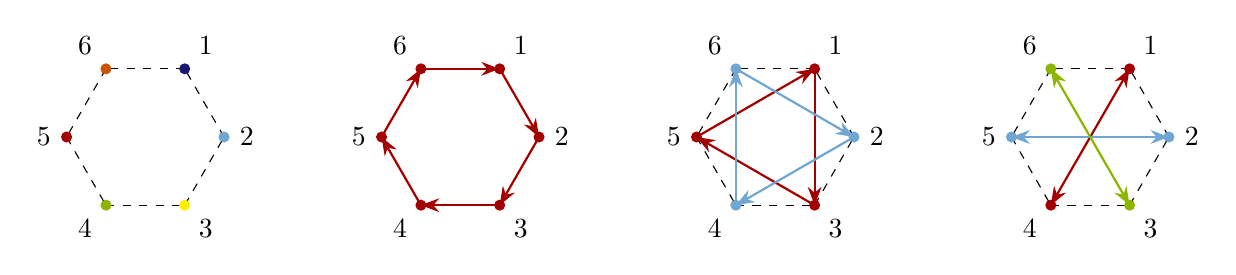
\begin{tikzpicture}[>=Stealth]
            \tikzstyle{point}=[circle,fill,inner sep=0pt, minimum width=4pt, minimum height=4pt]
            
            \begin{scope}[shift={(-4,0)}]
                % Vertices of a regular hexagon
                \coordinate (V1) at (1,0);
                \coordinate (V2) at (0.5,0.866);
                \coordinate (V3) at (-0.5,0.866);
                \coordinate (V4) at (-1,0);
                \coordinate (V5) at (-0.5,-0.866);
                \coordinate (V6) at (0.5,-0.866);

                % Edges as arrows (counter-clockwise)
                \draw[dashed] (V1) -- (V2);
                \draw[dashed] (V2) -- (V3);
                \draw[dashed] (V3) -- (V4);
                \draw[dashed] (V4) -- (V5);
                \draw[dashed] (V5) -- (V6);
                \draw[dashed] (V6) -- (V1);

                % Vertex labels
                \node[label=right:$2$,iceberg] at (V1)[point] {};
                \node[label=above right:$1$,midnightblue] at (V2)[point] {};
                \node[label=above left:$6$,burntorange] at (V3)[point] {};
                \node[label=left:$5$,darkcandyapplered] at (V4)[point] {};
                \node[label=below left:$4$,applegreen] at (V5)[point] {};
                \node[label=below right:$3$,canaryyellow] at (V6)[point] {};
            \end{scope}

            \begin{scope}[shift={(0,0)}]
                % Vertices of a regular hexagon
                \coordinate (V1) at (1,0);
                \coordinate (V2) at (0.5,0.866);
                \coordinate (V3) at (-0.5,0.866);
                \coordinate (V4) at (-1,0);
                \coordinate (V5) at (-0.5,-0.866);
                \coordinate (V6) at (0.5,-0.866);

                % Edges as arrows (counter-clockwise)
                \draw[<-,darkcandyapplered, thick] (V1) -- (V2);
                \draw[<-,darkcandyapplered, thick] (V2) -- (V3);
                \draw[<-,darkcandyapplered, thick] (V3) -- (V4);
                \draw[<-,darkcandyapplered, thick] (V4) -- (V5);
                \draw[<-,darkcandyapplered, thick] (V5) -- (V6);
                \draw[<-,darkcandyapplered, thick] (V6) -- (V1);

                % Vertex labels
                \node[label=right:$2$,darkcandyapplered] at (V1)[point] {};
                \node[label=above right:$1$,darkcandyapplered] at (V2)[point] {};
                \node[label=above left:$6$,darkcandyapplered] at (V3)[point] {};
                \node[label=left:$5$,darkcandyapplered] at (V4)[point] {};
                \node[label=below left:$4$,darkcandyapplered] at (V5)[point] {};
                \node[label=below right:$3$,darkcandyapplered] at (V6)[point] {};
            \end{scope}

            \begin{scope}[shift={(4,0)}]
                % Vertices of a regular hexagon
                \coordinate (V1) at (1,0);
                \coordinate (V2) at (0.5,0.866);
                \coordinate (V3) at (-0.5,0.866);
                \coordinate (V4) at (-1,0);
                \coordinate (V5) at (-0.5,-0.866);
                \coordinate (V6) at (0.5,-0.866);

                % Edges as arrows (counter-clockwise)
                \draw[->,darkcandyapplered, thick] (V2) -- (V6);
                \draw[->,darkcandyapplered, thick] (V6) -- (V4);
                \draw[->,darkcandyapplered, thick] (V4) -- (V2);
                \draw[->,iceberg, thick] (V1) -- (V5);
                \draw[->,iceberg, thick] (V5) -- (V3);
                \draw[->,iceberg, thick] (V3) -- (V1);
                \draw[dashed] (V1) -- (V2);
                \draw[dashed] (V2) -- (V3);
                \draw[dashed] (V3) -- (V4);
                \draw[dashed] (V4) -- (V5);
                \draw[dashed] (V5) -- (V6);
                \draw[dashed] (V6) -- (V1);

                % Vertex labels
                \node[label=right:$2$,iceberg] at (V1)[point] {};
                \node[label=above right:$1$,darkcandyapplered] at (V2)[point] {};
                \node[label=above left:$6$,iceberg] at (V3)[point] {};
                \node[label=left:$5$,darkcandyapplered] at (V4)[point] {};
                \node[label=below left:$4$,iceberg] at (V5)[point] {};
                \node[label=below right:$3$,darkcandyapplered] at (V6)[point] {};
            \end{scope}

            \begin{scope}[shift={(8,0)}]
                % Vertices of a regular hexagon
                \coordinate (V1) at (1,0);
                \coordinate (V2) at (0.5,0.866);
                \coordinate (V3) at (-0.5,0.866);
                \coordinate (V4) at (-1,0);
                \coordinate (V5) at (-0.5,-0.866);
                \coordinate (V6) at (0.5,-0.866);

                % Edges as arrows (counter-clockwise)
                \draw[<->,darkcandyapplered, thick] (V2) -- (V5);
                \draw[<->,iceberg, thick] (V1) -- (V4);
                \draw[<->,applegreen, thick] (V6) -- (V3);
                \draw[dashed] (V1) -- (V2);
                \draw[dashed] (V2) -- (V3);
                \draw[dashed] (V3) -- (V4);
                \draw[dashed] (V4) -- (V5);
                \draw[dashed] (V5) -- (V6);
                \draw[dashed] (V6) -- (V1);

                % Vertex labels
                \node[label=right:$2$,iceberg] at (V1)[point] {};
                \node[label=above right:$1$,darkcandyapplered] at (V2)[point] {};
                \node[label=above left:$6$,applegreen] at (V3)[point] {};
                \node[label=left:$5$,iceberg] at (V4)[point] {};
                \node[label=below left:$4$,darkcandyapplered] at (V5)[point] {};
                \node[label=below right:$3$,applegreen] at (V6)[point] {};
            \end{scope}
        \end{tikzpicture}
        \]
        Άρα, στο σύνολο προκύπτουν 
        \[
        \frac{1}{6}(q^6 + q^3 + 2q^2 + 2q)
        \]
        χρωματισμοί.
    \end{itemize}
\end{proof}

\begin{remark}
    To (3) είναι γνωστό ως \emph{Λήμμα Burnside}. Για την ιστορία γύρω από το όνομα δείτε τις σημειώσεις στο \cite[Κεφάλαιο~7]{StaEC2}. Με τη συζήτηση της Παραγράφου 1 κατά νου, παρατηρούμε ότι 
    \begin{align*}
        \sigma_\epsilon &= 
        \textcolor{midnightblue}{\cycle{1}}
        \textcolor{iceberg}{\cycle{2}}  
        \textcolor{canaryyellow}{\cycle{3}}  
        \textcolor{applegreen}{\cycle{4}}  
        \textcolor{darkcandyapplered}{\cycle{5}} 
        \textcolor{burntorange}{\cycle{6}}  \\
        \sigma_r &= 
        \textcolor{darkcandyapplered}{\cycle{1,2,3,4,5,6}} \\ 
        \sigma_{r^2} &= 
        \textcolor{darkcandyapplered}{\cycle{1,3,5}}
        \textcolor{iceberg}{\cycle{2,4,6}} \\ 
        \sigma_{r^3} &= 
        \textcolor{darkcandyapplered}{\cycle{1,4}}
        \textcolor{iceberg}{\cycle{2,5}}  
        \textcolor{applegreen}{\cycle{3,6}}. \\ 
    \end{align*}
    Αυτό δεν είναι σύμπτωση. Γενικότερα, αν $S$ είναι ένα $G$-σύνολο, τότε το πλήθος των μη ισοδύναμων (ως προς $G$) $q$-χρωματισμών του $S$ ισούται με 
    \[
    \frac{1}{\abs{G}} \sum_{g \in G} q^{\mathrm{c}(\sigma_g)},
    \]
    όπου $\mathrm{c}(\sigma_g)$ είναι το πλήθος των κύκλων στην κυκλική μορφή της $\sigma_g$.

    Στην περίπτωση της γνωστής μας δράσης καθορισμού της συμμετρικής ομάδας $\fS_n$ στο $[n]$, μπορεί να αποδείξει κανείς ότι, το πλήθος των μη ισοδύναμων $q$-χρωματισμών του $[n]$ ισούται με 
    \[
    \binom{q+n-1}{n} = \frac{1}{n!}q(q+1)\cdots(q+n-1).
    \] 
    Συνεπώς, προκύπτει η ταυτότητα
    \[
    \sum_{\pi \in \fS_n} q^{\mathrm{c}(\pi)} = q(q+1)\cdots(q+n-1).
    \]
    Οι συντελεστές του πολυωνύμου του αριστερού μέλους ονομάζονται \emph{αριθμοί Stirling πρώτου είδους}.
\end{remark}

\begin{exercise}{(\texttt{Αναμενώμενος αριθμός σταθερών σημείων μιας τυχαίας μετάθεσης})} 
    \label{ex:2.4}\\
    Να υπολογίσετε τα παρακάτω αθροίσματα
    \[
    \sum_{\pi \in \fS_n} \fix(\pi) \quad \text{και} \quad \sum_{\pi \in \fS_n} \fix(\pi)^2.
    \]
    Ποιός είναι ο αναμενώμενος αριθμός των σταθερών σημείων μιας τυχαίας μετάθεσης;
\end{exercise}

\begin{proof}[Λύση]
    Η δράση καθορισμού της $\fS_n$ στο $[n]$ είναι μεταβατική. Συνεπώς, από την Άσκηση \ref{ex:2.3} έπεται ότι 
    \[
    \frac{1}{n!}\sum_{\pi \in \fS_n} \fix(\pi) = 1.
    \]
    Επομένως, ο αναμενώμενος αριθμός των σταθερών σημείων μια τυχαίας μετάθεσης είναι ίσος με 1 και το πρώτο άθροισμα ισούται με $n!$.

    Για το δεύτερο άθροισμα, παρατηρούμε ότι 
    \[
    \frac{1}{n!}\sum_{\pi \in \fS_n} \fix(\pi)^2 = \left(
        \chi^\rmdef, \chi^\rmdef 
    \right) = 2,
    \]
    όπου η τελευταία ισότητα έπεται από το Παράδειγμα 6.8 και γι αυτό 
    \[
    \sum_{\pi \in \fS_n} \fix(\pi)^2 = 2n!.
    \]
\end{proof}

\begin{exercise}{(\texttt{Αθροίσματα γραμμών του πίνακα χαρακτήρων})} 
    \label{ex:2.5}\\
    Έστω $\psi_G$ ο χαρακτήρας της αναπαράστασης μεταθέσεων που επάγεται από τη δράση της $G$ στον εαυτό της με συζυγία. Να δείξετε τα εξής.
    \begin{itemize}
        \item[(1)] Έχουμε 
        \[
        \psi_G = \sum_{\chi}\chi\ol{\chi},
        \]
        όπου στο άθροισμα το $\chi$ διατρέχει όλους τους ανάγωγους χαρακτήρες της $G$.
        \item[(2)] Αν $\chi$ είναι ένας ανάγωγος χαρακτήρας της $G$, τότε
        \[
        (\, \psi_G, \chi \,) = \sum_K \chi(K),
        \]
        όπου στο άθροισμα το $K$ διατρέχει όλες τις κλάσεις συζυγίας της $G$.
        \item[(3)] Τα αθροίσματα των στοιχείων των γραμμών του πίνακα χαρακτήρων της $G$ είναι μη αρνητικοί αριθμοί.
    \end{itemize}
\end{exercise}

\begin{proof}[Λύση]
    \leavevmode
    \begin{itemize}
        \item[(1)]
        Για $g \in G$, έστω $\rmZ_g$ και $\rmK_g$ ο κεντρικοποιητής και η κλάση συζυγίας του $g$ στην $G$, αντίστοιχα. Από την Άσκηση \ref{ex:2.3} (1) 
        \[
        \psi_G(g) = \abs{\{
            x \in G : gxg^{-1} = x
        \}} = \abs{\rmZ_g} = \frac{\abs{G}}{\abs{\rmK_g}},
        \]
        όπου η τελευταία ισότητα έπεται από την Ταυτότητα (1.1). Το ζητούμενο έπεται από το Θεώρημα 7.9.
        \item[(3)] Το ζητούμενο έπεται από το Πόρισμα 7.5 και το (2).
    \end{itemize}
\end{proof}

\begin{remark}
    Στην περίπτωση της συμμετρικής ομάδας ισχύει επιπλέον ότι και τα αθροίσματα των στοιχείων των \emph{στηλών} του πίνακα χαρακτήρων της είναι μη αρνητικοί ακέραιοι. Πιο συγκεκριμένα, 
    \[
    \sum_{\lambda \vdash n} \chi^\lambda(\pi) = 
    \abs{
        \{
            \sigma \in \fS_n : \pi = \sigma^2
        \}
    }
    \]
    (βλ. \cite[Άσκηση~7.69]{StaEC2}). Για $\pi = \epsilon$, η ταυτότητα γίνεται 
    \[
    \sum_{\lambda \vdash n} f^\lambda = 
    \abs{
        \{
            \sigma \in \fS_n : \sigma^2 = \epsilon
        \}
    }.
    \]
    Οι μεταθέσεις που απαριθμούνται στο δεξί μέλος της παραπάνω ισότητας ονομάζονται \emph{αυτοαντίστροφες} (involutions). Συγκρίνετε με το Θεώρημα 12.6.
\end{remark}

\setcounter{section}{3}
\setcounter{exercise}{0}
\thispagestyle{empty}

\begin{exercise}{(\texttt{Χώρος πηλίκο ως αναπαράσταση})} 
    \label{ex:3.1}\\
    Έστω $\FF$ ένα σώμα, $V$ ένα $G$-πρότυπο και $W$ ένα υποπρότυπο του $V$. Να δείξετε τα εξής.
    \begin{itemize}
        \item[(1)] Ο (διανυσματικός) χώρος πηλίκο $V/W$ γίνεται $G$-πρότυπο θέτοντας 
        \[
        g \cdot\left(v + W\right) = gv + W
        \]
        για κάθε $g \in G$ και $v \in V$.
        \item[(2)] Έχουμε $V \cong_G W \oplus \left(V/W\right)$ (ως $G$-πρότυπα).
    \end{itemize}
\end{exercise}

\begin{exercise}{(\texttt{Ορίζουσα του πίνακα χαρακτήρων})} 
    \label{ex:3.2}\\
    Έστω $\rmK_1, \rmK_2, \dots, \rmK_r$ οι κλάσεις συζυγίας της $G$. Αν $X = (\chi(\rmK_j))_{\chi,j}$ είναι ο πίνακας χαρακτήρων της $G$, όπου το $\chi$ διατρέχει όλους τους διαφορετικούς ανάγωγους χαρακτήρες της $G$ και $1 \le j \le r$, τότε να δείξετε ότι 
    \[
    \abs{\det(X)}^2 = \frac{\abs{G}^r}{\abs{\rmK_1}\abs{\rmK_2}\cdots\abs{\rmK_r}}.
    \]
\end{exercise}

\begin{proof}[Λύση]
    Θεωρούμε τον πίνακα 
    \[
    Y = \left(
        \sqrt{\frac{\abs{\rmK_j}}{\abs{G}}}\chi(\rmK_j)
    \right)_{\chi, j},
    \]
    όπου το $\chi$ διατρέχει όλους τους διαφορετικούς ανάγωγους χαρακτήρες της $G$ και $1 \le j \le r$. Παρατηρούμε ότι 
    \[
    \det(Y) 
    = \det\left(X\begin{pmatrix}
        \sqrt{\frac{\abs{\rmK_1}}{\abs{G}}} & 0 & \cdots & 0 \\
        0 & \sqrt{\frac{\abs{\rmK_2}}{\abs{G}}} & \cdots & 0 \\
        \vdots & \vdots & & \vdots \\
        0 & 0 & \cdots & \sqrt{\frac{\abs{\rmK_r}}{\abs{G}}}
    \end{pmatrix}\right)
    = \det(X)\prod_{j=1}^r \sqrt{\frac{\abs{\rmK_j}}{\abs{G}}},
    \]
    όπου η δεύτερη ισότητα έπεται από την πολλαπλασιαστικότητα της ορίζουσας. Συνεπώς, 
    \begin{equation}
        \label{eq:3.2}
    \abs{\det(Y)}^2 = \abs{\det(X)}^2 \prod_{j=1}^r \frac{\abs{\rmK_j}}{\abs{G}}.
    \end{equation}

    Από την άλλη μεριά, από την απόδειξη του Θεωρήματος 7.9 γνωρίζουμε ότι $YY^\ast = \rmI_r$ και γι αυτό 
    \begin{align*}
    \abs{\det(Y)}^2 &= \det(Y)\ol{\det(Y)} \\
    &= \det(Y)\det(\ol{Y}) \\ 
    &= \det(Y)\det(\ol{Y}^\top) \\ 
    &= \det(Y)\det(Y^\ast) \\ 
    &= \det(YY^\ast) \\ 
    &= 1,
    \end{align*}
    όπου η τρίτη ισότητα έπεται από το ότι η ορίζουσα ενός πίνακας και του ανάστροφού του είναι ίσες. Το ζητούμενο έπεται από αυτή την παρατήρηση και την Ταυτότητα \eqref{eq:3.2}.
\end{proof}

\begin{remark}
    Γενικότερα, η ορίζουσα του πίνακα χαρακτήρων μιας πεπερασμένης ομάδας είναι είτε πραγματικός αριθμός, είτε μιγαδικός αριθμός με μηδενικό πραγματικό μέρος.
\end{remark}

\begin{exercise}{(\texttt{Εναλλαγή περιορισμού και επαγωγής})} 
    \label{ex:3.3}\\
    Έστω $H$ μια υποομάδα της $G$ και $\chi$ (αντ. $\psi$) ένας χαρακτήρας της $G$ (αντ. $H$). Να δείξετε ότι 
    \[
    \left(\psi \left(\chi\!\downarrow_H\right) \right)\!\uparrow^G = \psi\!\uparrow^G \chi.
    \]
\end{exercise}

\begin{proof}[Λύση]
    Αρχικά παρατηρούμε ότι αν $\alpha, \beta, \gamma$ είναι χαρακτήρες της $G$, τότε 
    \begin{equation}
        \label{eq:3.3}
    (\alpha\beta, \gamma) = (\alpha, \ol{\beta}\gamma).
    \end{equation}
    Πράγματι, υπολογίζουμε 
    \begin{align*}
        (\alpha\beta,\gamma) 
        &= \frac{1}{\abs{G}}\sum_{g \in G} (\alpha\beta)(g)\ol{\gamma(g)} \\
        &= \frac{1}{\abs{G}}\sum_{g \in G} \alpha(g)\beta(g)\ol{\gamma(g)} \\
        &= \frac{1}{\abs{G}}\sum_{g \in G} \alpha(g)\ol{\ol{\beta(g)}\gamma(g)} \\
        &= \frac{1}{\abs{G}}\sum_{g \in G} \alpha(g)\ol{\left(\ol{\beta}\gamma\right)(g)} \\
        &= (\alpha, \ol{\beta}\gamma).
    \end{align*}

    Πίσω στην λύση της άσκησης, επειδή το εσωτερικό γινόμενο $(\Arg,\Arg)_G$ είναι θετικά ορισμένο, αρκεί ν' αποδείξουμε ότι 
    \[
    \left(
        \left(\psi \left(\chi\!\downarrow_H\right) \right)\!\uparrow^G, \alpha
    \right) = 
    \left(
        \psi\!\uparrow^G \chi, \alpha
    \right)
    \] 
    για έναν αυθαίρετο χαρακτήρα $\alpha$ της $G$. Πράγματι, έστω $\alpha$ ένας χαρακτήρας της $G$. Από την μία μεριά, έχουμε 
    \[
    \left(
        \left(\psi\left(\chi\!\downarrow_H\right) \right)\!\uparrow^G, \alpha
    \right)_G = 
    \left(
        \psi \left(\chi\!\downarrow_H\right), \alpha\!\downarrow_H
    \right)_H = 
    \left(
        \psi, \ol{\chi\!\downarrow_H}\alpha\!\downarrow_H
    \right)_H =
    \left(
        \psi, \left(\ol{\chi}\alpha\right)\!\downarrow_H
    \right)_H,
    \]
    όπου η πρώτη ισότητα έπεται από το Θεώρημα 8.8 και η δεύτερη από την Ταυτότητα \eqref{eq:3.3}. Από την άλλη,
    \[
    \left(
        \psi\!\uparrow^G \chi, \alpha
    \right)_G = 
    \left(
        \psi\!\uparrow^G, \ol{\chi}\alpha
    \right)_G =
    \left(
        \psi, \left(\ol{\chi}\alpha\right)\!\downarrow_H
    \right)_H,
    \]
    όπου η πρώτη ισότητα έπεται από την Ταυτότητα \eqref{eq:3.3} και η δεύτερη ισότητα έπεται από το Θεώρημα 8.8.
\end{proof}

\begin{exercise}
    \label{ex:3.4}
    Έστω $\chi$ ένας χαρακτήρας του κέντρου $\rmZ(G)$ της $G$. Να δείξετε ότι 
    \[
    \chi\!\uparrow_{\rmZ(G)}^G(g) = 
    \begin{cases}
        \frac{\abs{G}}{\abs{\rmZ(G)}}\,\chi(g), &\ \text{αν $g \in \rmZ(G)$} \\
        0, &\ \text{διαφορετικά}
    \end{cases}
    \]
    για κάθε $g \in G$.
\end{exercise}

\begin{proof}[Λύση]
    Έστω $g \in \rmZ(G)$. Τότε, $x^{-1}gx=g$ για κάθε $x \in G$. Από την Πρόταση 8.5 έπεται ότι 
    \[
        \chi\!\uparrow_{\rmZ(G)}^G(g) 
        = \frac{1}{\abs{\rmZ(G)}} \sum_{\substack{x \in G \\ x^{-1}gx\,\in\,\rmZ(G)}} \chi(x^{-1}gx) 
        = \frac{1}{\abs{\rmZ(G)}} \sum_{x \in G} \chi(g) \
        = \frac{\abs{G}}{\abs{\rmZ(G)}}\,\chi(g).
    \]

    Έστω $g \notin \rmZ(G)$. Θα δείξουμε ότι δεν υπάρχει $x \in G$ τέτοιο ώστε $x^{-1}gx \in \rmZ(G)$ και κατά συνέπεια $\chi\!\uparrow_{\rmZ(G)}^G(g) = 0$ από την Πρόταση 8.5. Έστω, λοιπόν, $x \in G$ τέτοιο ώστε $x^{-1}gx \in \rmZ(G)$. Τότε 
    \[
    y^{-1}gy = y^{-1}x(x^{-1}gx)x^{-1}y = \left(y^{-1}x\right)\,\left(x^{-1}gx\right)\,\left(y^{-1}x\right)^{-1} = x^{-1}gx,
    \]
    για κάθε $y \in G$. Άρα, 
    \[
    \left(xy^{-1}\right)\,g\,\left(xy^{-1}\right)^{-1} = g
    \]
    για κάθε $y \in G$, ή ισοδύναμα, $hgh^{-1} = g$ για κάθε $h \in G$, το οποίο είναι αδύνατο.
\end{proof}

\begin{exercise}{(\texttt{Σχέσεις Coxeter})}
    \label{ex:3.5} \\
    Έστω $s_i \coloneqq \cycle{i, i+1}$, για κάθε $1 \le i \le n-1$ και $\epsilon$ η ταυτοτική μετάθεση. Να δείξετε τα εξής.
    \begin{itemize}
        \item[(1)] Το σύνολο $\{s_1, s_2, \dots, s_{n-1}\}$ παράγει την $\fS_n$.
    \item[(2)] Οι γειτονικές αντιμεταθέσεις ικανοποιούν τις σχέσεις 
    \begin{align*}
    s_i^2 &= \epsilon,  \hspace{-70pt}& &\text{για κάθε $1 \le i \le n-1$}\\
    s_is_{i+1}s_i &= s_{i+1}s_is_{i+1}, \hspace{-70pt}&  &\text{για κάθε $1 \le i \le n-2$} \\
    s_is_j &= s_js_i, \hspace{-70pt}&  &\text{για κάθε $\abs{i-j}>1$}. 
    \end{align*}
    \end{itemize}
\end{exercise}

\begin{proof}[Λύση]
    Στην Παράγραφο 9 είδαμε ότι η συμμετρική ομάδα παράγεται από το σύνολο όλων των αντιμεταθέσεων. Επομένως, για το (1), αρκεί να δείξουμε ότι κάθε αντιμετάθεση $\cycle{i,j}$ με $i > j$ μπορεί να γραφεί ως γινόμενο γειτονικών αντιμεταθέσεων. 
    
    Θα κάνουμε επαγωγή ως προς $j-i$. Αν $j-i = 1$, τότε $\cycle{i,j} = s_i$. Αυτή είναι η βάση της επαγωγής. Υποθέτουμε τώρα ότι η $\cycle{i,j}$ γράφεται ως γινόμενο γειτονικών αντιμεταθέσεων. Από την Πρόταση 9.2, 
    \[
    s_j\cycle{i,j}s_j^{-1} = \cycle{j,s_j(j)} = \cycle{i, j+1}.
    \]
    Συνεπώς, από την επαγωγική υπόθεση έπεται ότι η $\cycle{i, j+1}$ γράφεται ως γινόμενο γειτονικών αντιμεταθέσεων και το ζητούμενο έπεται.
\end{proof}

\begin{remark}
    Γενικότερα, αποδεικνύεται ότι η $\fS_n$ παράγεται ως ομάδα από το σύνολο $\{s_1,$ $s_2, \dots, s_{n-1}\}$ με σχέσεις αυτές που περιγράφονται στο (2). Αυτή είναι η παράσταση της συμμετρικής ομάδας ως \emph{ομάδας Coxeter}. Οι (πεπερασμένες) ομάδες Coxeter συμπίπτουν με τις ομάδες ανακλάσεων Ευκλείδιων χώρων και περιλαμβάνουν, για παράδειγμα, τις διεδρικές ομάδες καθώς και τις ομάδες συμμετρίας των κανονικών πολυέδρων. Πρόκειται για πολύ πλούσια συνδυαστικά αντικείμενα, που παίζουν κεντρικό ρόλο στην συνδυαστική και την θεωρία αναπαραστάσεων (βλ. \cite[Μέρος~III]{PetEN}).
\end{remark}

\begin{exercise}{(\texttt{Αντιστροφές και πρόσημο})} 
    \label{ex:3.6} \\
    Για $\pi \in \fS_n$, το ζεύγος $(i,j)$ με $1 \le i < j \le n$ τέτοια ώστε $\pi(i) > \pi(j)$ ονομάζεται \emph{αντιστροφή} (inversion) της $\pi$. Έστω $\Inv(\pi)$ το σύνολο όλων των αντιστροφών της $\pi$ και $\inv(\pi) \coloneqq \abs{\Inv(\pi)}$. Να δείξετε τα εξής.
    \begin{itemize}
        \item[(1)] Αν $s_i$ όπως στην Άσκηση~\ref{ex:3.5}, τότε
        \[
        \inv(\pi s_i) = 
        \begin{cases}
            \inv(\pi) + 1, &\ \text{αν $\pi_i < \pi_{i+1}$} \\
            \inv(\pi) - 1, &\ \text{αν $\pi_i > \pi_{i+1}$} \\
        \end{cases}
        \]
        για κάθε $1 \le i \le n-1$ και $\pi \in \fS_n$.
        \item[(2)] Κάθε $\pi \in \fS_n$ μπορεί να γραφεί ως γινόμενο $\inv(\pi)$ το πλήθος γειτονικών αντιμεταθέσεων.
        \item[(3)] Για κάθε $\pi \in \fS_n$, 
        \[
        \sign(\pi) = (-1)^{\inv(\pi)}.
        \]
        \item[(4)] Για κάθε $\pi, \sigma \in \fS_n$, 
        \begin{align*}
            \sign(\pi\sigma) &= \sign(\pi)\sign(\sigma) \\
            \sign(\pi^{-1}) &= \sign(\pi). \\
        \end{align*}
        \item[(5)] Ένας $k$-κύκλος είναι άρτιος αν και μόνο αν το $k$ είναι περιττός.
    \end{itemize}
\end{exercise}

\begin{proof}[Λύση]
    \leavevmode
    \begin{itemize}
        \item[(1)] Παρατηρούμε ότι η μετάθεση $\pi s_i$ διαφέρει από την $\pi$ μόνο στις θέσεις $i$ και $i+1$. Συνεπώς, αν $\pi_i < \pi_{i+1}$, τότε 
        \[
        \Inv(\pi s_i) = \Inv(\pi) \cup \{(i, i+1)\},
        \]
        ενώ αν $\pi_i > \pi_{i+1}$, τότε 
        \[
        \Inv(\pi s_i) = \Inv(\pi) \setminus \{(i, i+1)\}.
        \]
        και το ζητούμενο έπεται.
        \item[(2)] Θα κάνουμε επαγωγή ως προς $\inv(\pi)$. Αν $\inv(\pi) = 0$, τότε $\pi = \epsilon$. Αυτή είναι η βάση της επαγωγής. Υποθέτουμε τώρα ότι $\inv(\pi) > 0$ και ότι κάθε μετάθεση $\sigma \in \fS_n$ με $\inv(\sigma) < \inv(\pi)$ μπορεί να γραφεί ως γινόμενο $\inv(\sigma)$ το πλήθος γειτονικών αντιμεταθέσεων. 
        
        Θεωρούμε $1 \le i \le n-1$ τέτοιο ώστε $\pi_i > \pi_{i+1}$. Τέτοιος δείκτης $i$ υπάρχει, διότι σε διαφορετική περίπτωση $\pi_1 < \pi_2 < \cdots < \pi_n$ που σημαίνει ότι $\inv(\pi) = 0$, το οποίο είναι αδύνατο. Από το (1) έπεται ότι 
        \[
        \inv(\pi s_i) = \inv(\pi) - 1
        \]
        και γι αυτό από την επαγωγική υπόθεση,
        \[
        \pi s_i = s_{i_1}s_{i_2}\cdots s_{i_{\inv(\pi)}-1}
        \]
        που σημαίνει ότι 
        \[
        \inv(\pi s_i) = s_{i_1}s_{i_2}\cdots s_{i_{\inv(\pi)}-1}s_i
        \]
        και το ζητούμενο έπεται.

        \item[(3)] Θα κάνουμε επαγωγή ως προς $\inv(\pi)$. Αν $\inv(\pi) = 0$, τότε $\pi = \epsilon$ και γι αυτό $\sign(\pi) = 1 = (-1)^0$. Αυτή είναι η βάση της επαγωγής. Υποθέτουμε τώρα ότι $\inv(\pi) > 0$ και ότι κάθε μετάθεση $\sigma \in \fS_n$ με $\inv(\sigma) < \inv(\pi)$ ικανοποιεί 
        \[
        \sign(\sigma) = (-1)^{\inv(\sigma)}.
        \]
        
        Από το (2), μπορούμε να γράψουμε 
        \[
        \pi = \underbrace{s_{i_1}s_{i_2}\cdots s_{i_{\inv(\pi)}-1}}_{= \, \sigma}s_i. 
        \]
        Από το (1) έπεται ότι $\inv(\pi) = \inv(\sigma) \pm 1$ και γι αυτό 
        \[
        \inv(\pi) \equiv \inv(\sigma) + 1 \pmod{2}.
        \]
        Συνεπώς, από την επαγωγική υπόθεση έχουμε 
        \[
        \sign(\pi) = (-1)^{\inv(\sigma) + 1} = (-1)^{\inv(\pi)}
        \]
        και το ζητούμενο έπεται.

        \item[(4)] Αρκεί να παρατηρήσει κανείς ότι 
        \[
        \inv(\pi\sigma) \equiv \inv(\pi) + \inv(\sigma) \pmod{2}.
        \]
    \end{itemize}
\end{proof}

\begin{remark}
    Το $\inv$ είναι μια ακόμα στατιστική μεταθέσεων. Αποδεικνύεται ότι 
    \[
    \sum_{\pi \in \fS_n} q^{\inv(\pi)} = (1+q)(1+q+q^2)\cdots(1+q+q^2+ \cdots + q^{n-1}).
    \]
    Ένας δέικτης $1 \le i \le n-1$ για τον οποίο $\pi_i > \pi_{i+1}$ ονομάζεται \emph{κάθοδος} (descent) της $\pi$. Το σύνολο (αντ. πλήθος) όλων των καθόδων της $\pi$ συμβολίζεται με $\Des(\pi)$ (αντ. $\des(\pi)$). Το πολυώνυμο
    \[
    A_n(t) \coloneqq \sum_{\pi \in \fS_n} t^{\des(\pi)}
    \] 
    που \textquote{καταγράφει} την κατανομή του πλήθους των καθόδων πάνω από την $\fS_n$ ονομάζεται \emph{$n$-οστό πολυώνυμο του Euler} και αποτελεί ένα από τα πιο σημαντικά πολυώνυμα στην τομή της συνδυαστικής, της άλγεβρας και της γεωμετρίας (βλ. \cite{PetEN}). 

    Αποδεικνύεται ότι $\inv(\pi)$ είναι το ελάχιστο πλήθος γειτονικών αντιστροφών που μπορούμε να κάνουμε στις εισόδους της $\pi$ έτσι ώστε να την μετασχηματίσουμε στην ταυτοτική μετάθεση. Κάθε έκφραση της μορφής 
    \[
    \pi = s_{i_1}s_{i_2} \cdots s_{i_{\inv(\pi)}}
    \]
    ονομάζεται \emph{reduced expression} της $\pi$. Μια μετάθεση μπορεί να έχει πολλές διαφορετικές τέτοιες εκφράσεις. Ο Stanley το 1984 απέδειξε ότι το πλήθος των reduced expressions της μετάθεσης $n(n-1)\cdots21$\footnote{Αυτή είναι η μετάθεση με τις περισσότερες αντιστροφές ανάμεσα στις μεταθέσεις της $\fS_n$.} ισούται με το πλήθος των συνήθων Young ταμπλώ σχήματος $\delta_n$ που συναντήσαμε στην Παράγραφο 18 (βλ., για παράδειγμα, \cite[Άσκηση~7.22~(f)]{StaEC2}), δίνοντας έτσι μια ερμηνεία ως διάστασης μιας ανάγωγης αναπαράστασης της $\fS_n$.
\end{remark}

\setcounter{section}{4}
\setcounter{exercise}{0}
\thispagestyle{empty}

\begin{exercise}{(\texttt{Πίνακας χαρακτήρων της $\fS_4$ (ξανά)})} 
    \label{ex:4.1}\\
    Για $\lambda \vdash n$, έστω $\rho^\lambda : \fS_n \to \GL_{f^\lambda}(\CC)$ η αναπαράσταση της $\fS_n$ που αντιστοιχεί στο πρότυπο Specht $\sS^\lambda$ και $\chi^\lambda$ ο χαρακτήρας της. Υποθέτουμε ότι $n=4$.
    \begin{itemize}
        \item[(1)] Για κάθε $\lambda \vdash 4$, να βρείτε τις τιμές του χαρακτήρα $\chi^\lambda$ υπολογίζοντας τους πίνακες $\rho^\lambda(\pi)$, για κάθε $\pi \in \fS_4$, στην βάση $\{\bfe_T : T \in \SYT(\lambda)\}$.
        \item[(2)] Χρησιμοποιώντας το (1), γράψτε τον πίνακα χαρακτήρων της $\sS_4$.
    \end{itemize}
\end{exercise}

\begin{proof}[Λύση]
    To Θεώρημα 12.3 μας πληροφορεί ότι
    \[ 
    \dim(\sS^\lambda) = f^\lambda.
    \]
    Χρησιμοποιώντας το Θεώρημα 12.8 υπολογίζουμε:
    \[
    \renewcommand{\arraystretch}{1.2}
    \begin{array}{c|c|c|c|c|c}
        \lambda   & (1,1,1,1) & (2,1,1) & (2,2) & (3,1) & (4) \\\hline
        f^\lambda & 1         & 3       & 2     & 3     & 1 
    \end{array} \ .
    \]

    Για $\lambda \in \{(1^4), (4)\}$ έχουμε
    \[
    \ytableausetup{smalltableaux,centertableaux}
    \sS^{1^4} = \CC[\,\bfe_{\ytableaushort{1,2,3,4}}\,], \quad \text{και} \quad 
    \sS^{(4)} = \CC[\,\bfe_{\ytableaushort{1234}}\,].
    \]
    Στο Παράδειγμα 11.3 είδαμε ότι αυτά είναι ισόμορφα με το πρότυπο προσήμου και το πρότυπο της τετριμμένης αναπαράστασης αντίστοιχα. Γι αυτό, 
    \[
    \renewcommand{\arraystretch}{1.2}
    \begin{array}{c|c|c|c|c|c}
                     & \rmK_{(1^4)} & \rmK_{211}  & \rmK_{22}              & \rmK_{31} & \rmK_4 \\ \hline
        \pi          & \epsilon     & \cycle{1,2} & \cycle{1,2}\cycle{3,4} & \cycle{1,2,3}      & \cycle{1,2,3,4} \\ \hline
        \chi^{(1^4)}(\pi) & 1            & -1          & 1                              & 1         & -1 \\ \hline 
        \chi^{(4)}(\pi) & 1            & 1          & 1                              & 1         & 1 
    \end{array} \ .
    \]

    Για τις υπόλοιπες $\lambda$, αρκεί να υπολογίσουμε τους πίνακες $\rho^\lambda(\cycle{1,2}), \rho^\lambda(\cycle{2,3})$ και $\rho^\lambda(\cycle{3,4})$. Πράγματι, η Άσκηση \ref{ex:3.5} μας πληροφορεί ότι η $\fS_4$ παράγεται από τα $\cycle{1,2}, \cycle{2,3}$ και $\cycle{3,4}$ και επειδή η $\rho^\lambda$ είναι ομομορφισμός ομάδων, για να υπολογίσουμε τους $\rho^\lambda(\pi)$, αρκεί να γράψουμε κάθε $\pi \in \fS_4$ ως γινόμενο γειτονικών αντιμεταθέσεων και έπειτα να πολλαπλασιάσουμε τους αντίστοιχους πίνακες.
    
    Για $\lambda = (2,1,1)$, έχουμε
    \[
    \ytableausetup{smalltableaux,centertableaux}
    \sS^{211} = \CC[
        \,\bfe_{\ytableaushort{12,3,4}}\, ,
        \,\bfe_{\ytableaushort{13,2,4}}\, ,
        \,\bfe_{\ytableaushort{14,2,3}}\,
        ].
    \]
    Ως προς την βάση αυτή υπολογίζουμε:
    \begin{align*}
        \rho^{211}(\cycle{1,2}) &= 
        \begin{pmatrix}
            1  & 0  & 0 \\
            -1 & -1 & 0 \\
            1  & 0  & -1
        \end{pmatrix} \\
        \rho^{211}(\cycle{2,3}) &=
        \begin{pmatrix}
            0 & 1 & 0 \\
            1 & 0 & 0 \\
            0 & 0 & -1
        \end{pmatrix} \\ 
        \rho^{211}(\cycle{3,4}) &=
        \begin{pmatrix}
            -1 & 0 & 0 \\ 
            0  & 0 & 1 \\
            0 & 1 & 0 
        \end{pmatrix}
    \end{align*}
    και γι αυτό 
    \[
    \renewcommand{\arraystretch}{1.2}
    \begin{array}{c|c|c|c|c|c}
                        & \rmK_{(1^4)} & \rmK_{211}  & \rmK_{22}              & \rmK_{31} & \rmK_4 \\ \hline
        \pi             & \epsilon     & \cycle{1,2} & \cycle{1,2}\cycle{3,4} & \cycle{1,2,3}      & \cycle{1,2,3,4} \\ \hline
        \rho^{211}(\pi) & \begin{pmatrix}
            1 & 0 & 0 \\
            0 & 1 & 0 \\ 
            0 & 0 & 1
        \end{pmatrix}             & \begin{pmatrix}
            1 & 0 & 0 \\
            -1 & -1 & 0 \\
            1 & 0 & -1 
        \end{pmatrix}          & \begin{pmatrix}
            -1 & 0 & 0 \\
            1 & 0 & -1 \\
            -1 & -1 & 0
        \end{pmatrix}                              & \begin{pmatrix}
            0 & 1 & 0 \\
            -1 & -1 & 0 \\
            0 & 1 & 1 
        \end{pmatrix}         & \begin{pmatrix}
            0 & 0 & 1 \\
            1 & 0 & -1 \\
            0 & 1 & 1
        \end{pmatrix}  \\ \hline
        \chi^{211}(\pi) & 3            & -1          & -1                              & 0         & 1 
    \end{array} \ .
    \]

    Για $\lambda = (2,2)$, έχουμε 
    \[
    \ytableausetup{smalltableaux,centertableaux}
    \sS^{211} = \CC[
        \,\bfe_{\ytableaushort{12,34}}\, ,
        \,\bfe_{\ytableaushort{13,24}}\,
        ].
    \]
    Ως προς την βάση αυτή υπολογίζουμε:
    \begin{align*}
        \rho^{22}(\cycle{1,2}) &= 
        \begin{pmatrix}
            1  & 0  \\
            -1 & -1
        \end{pmatrix} \\
        \rho^{22}(\cycle{2,3}) &=
        \begin{pmatrix}
            0 & 1 \\
            1 & 0 
        \end{pmatrix} \\ 
        \rho^{22}(\cycle{3,4}) &=
        \begin{pmatrix}
            1 & 0 \\ 
            -1  & -1
        \end{pmatrix}
    \end{align*}
    και γι αυτό 
    \[
    \renewcommand{\arraystretch}{1.2}
    \begin{array}{c|c|c|c|c|c}
                        & \rmK_{(1^4)} & \rmK_{211}  & \rmK_{22}              & \rmK_{31} & \rmK_4 \\ \hline
        \pi             & \epsilon     & \cycle{1,2} & \cycle{1,2}\cycle{3,4} & \cycle{1,2,3}      & \cycle{1,2,3,4} \\ \hline
        \rho^{22}(\pi) & \begin{pmatrix}
            1 & 0 \\
            0 & 1
        \end{pmatrix}             & \begin{pmatrix}
            1 & 0 \\
            -1 & -1 
        \end{pmatrix}          & \begin{pmatrix}
            1 & 0  \\
            0 & 1 
        \end{pmatrix}                              & \begin{pmatrix}
            0 & 1 \\
            -1 & -1 
        \end{pmatrix}         & \begin{pmatrix}
            -1 & -1 \\
            1 & 1 
        \end{pmatrix}  \\ \hline
        \chi^{22}(\pi) & 2  & 0  & 2  & -1  & 0
    \end{array} \ .
    \]

    Για $\lambda = (3,1)$, έχουμε
    \[
    \ytableausetup{smalltableaux,centertableaux}
    \sS^{31} = \CC[
        \,\bfe_{\ytableaushort{134,2}}\, ,
        \,\bfe_{\ytableaushort{124,3}}\, ,
        \,\bfe_{\ytableaushort{123,4}}\,
        ].
    \]
    Ως προς την βάση αυτή υπολογίζουμε:
    \begin{align*}
        \rho^{31}(\cycle{1,2}) &= 
        \begin{pmatrix}
            1 & -1 & -1 \\
            0 & 1  & 0 \\
            0 & 0  & 1
        \end{pmatrix} \\
        \rho^{31}(\cycle{2,3}) &=
        \begin{pmatrix}
            0 & 1 & 0 \\
            1 & 0 & 0 \\
            0 & 0 & 1
        \end{pmatrix} \\ 
        \rho^{31}(\cycle{3,4}) &=
        \begin{pmatrix}
            1 & 0 & 0 \\ 
            0  & 0 & 1 \\
            0 & 1 & 0 
        \end{pmatrix}
    \end{align*}
    και γι αυτό 
    \[
    \renewcommand{\arraystretch}{1.2}
    \begin{array}{c|c|c|c|c|c}
                        & \rmK_{(1^4)} & \rmK_{211}  & \rmK_{22}              & \rmK_{31} & \rmK_4 \\ \hline
        \pi             & \epsilon     & \cycle{1,2} & \cycle{1,2}\cycle{3,4} & \cycle{1,2,3}      & \cycle{1,2,3,4} \\ \hline
        \rho^{31}(\pi) & \begin{pmatrix}
            1 & 0 & 0 \\
            0 & 1 & 0 \\ 
            0 & 0 & 1
        \end{pmatrix}             & \begin{pmatrix}
            -1 & -1 & -1 \\
            0 & 1 & 0 \\
            0 & 0 & 1 
        \end{pmatrix}          & \begin{pmatrix}
            -1 & -1 & -1 \\
            0 & 0 & 1 \\
            0 & 1 & 0
        \end{pmatrix}                              & \begin{pmatrix}
            -1 & -1 & -1 \\
            1 & 0 & 0 \\
            0 & 0 & 1 
        \end{pmatrix}         & \begin{pmatrix}
            -1 & -1 & -1 \\
            1 & 0 & 0 \\
            0 & 1 & 0
        \end{pmatrix}  \\ \hline
        \chi^{31}(\pi) & 3 & 1  & -1 & 0 & -1 
    \end{array} \ .
    \]

    Ο πίνακας χαρακτήρων της $\fS_4$ είναι 
    \[
    \renewcommand{\arraystretch}{1.2} 
    \begin{array}{c|c|c|c|c|c}
               & \rmK_{1111}  & \rmK_{211}  & \rmK_{22} & \rmK_{31} & \rmK_4  \\ \hline
    \chi^{4} & 1            & 1           & 1         & 1         & 1 \\ \hline 
    \chi^{1^4} & 1            & -1          & 1         & 1         & -1 \\ \hline 
    \chi^{31}  & 3            & 1           & -1        & 0         & -1  \\ \hline 
    \chi^{211}     & 3            & -1          & -1        & 0         & 1 \\ \hline 
    \chi^{22}     & 2            & 0           & 2         & -1        & 0
    \end{array}\ .
    \]
\end{proof}

\begin{remark}
    Συγκρίνοντας με τον υπολογισμό του πίνακα χαρακτήρων που κάναμε στο μάθημα, παρατηρούμε ότι 
    \[
    \sS^{211} \cong_{\fS_4} \sS^{31}\otimes\sS^{1^4},
    \]
    σε συμφωνία με την Άσκηση \ref{ex:5.3}. 
\end{remark}

\begin{exercise}
    \label{ex:4.2}
    Έστω $\Pi_4$ το σύνολο όλων των διαμερίσεων του $[4]$. Να υπολογίσετε την ισοτυπική διάσπαση της αναπαράστασης μεταθέσεων που επάγεται από τη δράση καθορισμού της $\fS_4$ στο $\Pi_4$.
\end{exercise}

\begin{proof}[Λύση]
    Για $B \in \Pi_n$, έστω $\lambda(B)$ η διαμέριση του $n$ που προκύπτει αναδιατάσσοντας τα μέρη της $B$ σε ασθενώς φθίνουσα σειρά ως προς τα μήκη των μερών της. Για $\lambda \vdash n$, έστω 
    \[
    \Pi_n^\lambda \coloneqq \{B \in \Pi_n : \lambda(B) = \lambda\},
    \]
    το οποίο γίνεται $\fS_n$-πρότυπο με τον προφανή τρόπο. Έχουμε την ακόλουθη διάσπαση $\fS_n$-προτύπων 
    \[
    \CC[\Pi_n] = \bigoplus_{\lambda \vdash n} \CC[\Pi_n^\lambda].
    \]

    Για $n=4$, η διάσπαση αυτή παίρνει την μορφή 
    \[
    \CC[\Pi_4] = \CC[\Pi_4^{4}] \oplus \CC[\Pi_4^{31}] \oplus \CC[\Pi_4^{22}] \oplus \CC[\Pi_4^{211}] \oplus \CC[\Pi_4^{1^4}].
    \]
    Για $\lambda \in \{(4), (1^4)\}$, έχουμε 
    \[
    \CC[\Pi_4^{4}] = \CC[1234] \quad \text{και} \quad 
    \CC[\Pi_4^{1^4}] = \CC[1\vert2\vert3\vert4],
    \]
    αντίστοιχα. Τα πρότυπα αυτά είναι και τα δυο ισόμορφα με το πρότυπο της τετριμμένης αναπαράστασης και γι αυτό 
    \[
    \CC[\Pi_4^{4}] \cong \CC[\Pi_4^{1^4}] \cong \sS^4.
    \]
    Στο μάθημα έχουμε δει ότι 
    \[
    \Pi_4^{22} = \sS^{4} \oplus \sS^{22}.
    \]

    Αν $\phi_4^{22}$ και $\phi_4^{31}$ είναι οι χαρακτήρες των αναπαραστάσεων μεταθέσεων $\CC[\Pi_4^{22}]$ και $\CC[\Pi_4^{31}]$, αντίστοιχα, τότε χρησιμοποιώντας το (1) της Άσκησης \ref{ex:2.3}, υπολογίζει κανείς 
    \[
    \renewcommand{\arraystretch}{1.2} 
    \begin{array}{c|c|c|c|c|c}
               & \rmK_{1111}  & \rmK_{211} & \rmK_{22} & \rmK_{31} & \rmK_4  \\ \hline
    \phi_4^{22} & 4           & 2          & 0         & 1         & 0 \\ \hline 
    \phi_4^{31} & 6           & 2          & 2         & 0         & 0 
    \end{array}\ .
    \]
    Τώρα, χρησιμοποιώντας το Πόρισμα 7.5 βρίσκει κανείς ότι 
    \begin{align*}
        \phi_4^{22} &= \chi^4 + \chi^{31} \\
        \phi_4^{22} &= \chi^4 + \chi^{31} + \chi^{22}. 
    \end{align*}

    Συμπερασματικά, το $\CC[\Pi_4^\lambda]$ είναι ισόμορφο με
    \[
    \begin{cases}
        \sS^4, &\ \text{αν $\lambda = (4)$} \\
        \sS^4\oplus\sS^{31}, &\ \text{αν $\lambda = (3,1)$} \\
        \sS^4\oplus\sS^{22}, &\ \text{αν $\lambda = (2,2)$} \\
        \sS^4\oplus\sS^{31}\oplus\sS^{22}, &\ \text{αν $\lambda = (2,1,1)$} \\
        \sS^4, &\ \text{αν $\lambda = (1,1,1,1)$}
    \end{cases}
    \]
    και γι αυτό η ζητούμενη ισοτυπική διάσπαση είναι
    \[
    \CC[\Pi_4] \cong_{\fS_4} \left(\sS^4\right)^5 \oplus \left(\sS^{31}\right)^2 \oplus \left(\sS^{22}\right)^2.
    \]
\end{proof}

\begin{remark}
    Παρατηρούμε ότι η πολλαπλότητα του προτύπου της τετριμμένης αναπαράστασης στην ισοτυπική διάσπαση του $\CC[\Pi_4]$ ισούται με 5, δηλαδή το πλήθος των τροχιών της δράσης της $\fS_4$ στο $\Pi_4$. Γενικότερα, αν $S$ είναι ένα $G$-σύνολο, τότε 
    \[
    (\chi^\triv, \CC[S]) \ = \ \text{πλήθος τροχιών της δράσης της $G$ στο $S$}.
    \]
\end{remark}

\begin{exercise}
\label{ex:4.3}
    Έστω $1 \le k \le n/2$ και $S$ το σύνολο όλων των υποσυνόλων του $[n]$ με $k$ στοιχεία. 
    \begin{itemize}
        \item[(1)] Να δείξετε ότι το πρότυπο Young $\rmM^{(n-k,k)}$ είναι ισόμορφο με το πρότυπο της αναπαράστασης μεταθέσεων που επάγεται από τη δράση καθορισμού της $\fS_n$ στο $S$.
        \item[(2)] Να υπολογίσετε το $f^{(n-k,k)}$, χωρίς να χρησιμοποιήσετε την hook-length formula.
        \item[(3)] Συμπεράνετε ότι $f^{(n,n)} = \frac{1}{n+1}\binom{2n}{n}$.
    \end{itemize}
\end{exercise}

\begin{proof}[Λύση]
    \leavevmode
    \begin{itemize}
        \item[(1)] Κάθε ταμπλοειδές σχήματος $(n-k,k)$ καθορίζεται από τα στοιχεία της δεύτερης γραμμής. Για $1 \le s_1 < s_2 < \cdots < s_k \le n$, θεωρούμε την απεικόνιση 
        \[
        \ytableausetup{tabloids}
        \begin{ytableau}
            \ast  & \ast & \cdots & \ast & \ast & \ast & \ast \\
            s_1   & s_2  & \cdots & s_k
        \end{ytableau} \ \mapsto \
        \{s_1, s_2, \dots, s_k\}.
        \]
        Αυτή είναι ο ζητούμενος $\fS_n$-ισομορφισμός.

        \item[(2)] Παρατηρούμε ότι  
        \[
        \rmK_{\lambda \, (n-k,k)} = 
        \begin{cases}
            1, &\ \text{αν $\lambda \in \{(n), (n-1,1), (n-2,2), \dots, (n-k,k)\}$} \\
            0, &\ \text{διαφορετικά}
        \end{cases}.
        \]
        Για παράδειγμα, για $n=6$ και $k=2$, έχουμε τα εξής ημισυνήθη ταμπλώ 
        \[
        \ytableausetup{nosmalltableaux,notabloids}
        \ytableaushort{111122}\, , \quad 
        \ytableaushort{11112,2}\, , \quad \text{και} \quad 
        \ytableaushort{1111,22}\, , 
        \]
        σχήματος $(6), (5,1)$ και $(4,2)$, αντίστοιχα. Συνεπώς, από το Θεώρημα 16.2 έπεται ότι
        \[
        \rmM^{(n-k,k)} \cong_{\fS_n} \rmM^{(n-k-1,k-1)} \oplus \sS^{(n-k,k)},
        \]
        ή ισοδύναμα 
        \[
        \chi^{(n-k,k)} = \varphi^{(n-k,k)} - \varphi^{(n-k-1,k-1)}
        \]
        από την Ταυτότητα~(6.2). Yπολογίζοντας την παραπάνω ταυτότητα στο ταυτοτικό στοιχείο της $\fS_n$ και χρησιμοποιώντας το (1)  προκύπτει ότι 
        \begin{equation}
            \label{eq:4.3}
            f^{(n-k,k)} = \binom{n}{k} - \binom{n}{k-1}.
        \end{equation}

        Διαφορετικά, θα αποδείξουμε την Ταυτότητα \eqref{eq:4.3} με επαγωγή στο $n$. Για $n=2$ και $k=1$, έχουμε $f^{(1,1)} = 1$. Αυτή είναι η βάση της επαγωγής. Υποθέτουμε ότι η Ταυτότητα \eqref{eq:4.3} ισχύει για $n-1$. Aπό την Πρόταση 13.2 έπεται ότι 
        \[
        f^{(n-k,k)} = f^{(n-k-1,k)} + f^{(n-k,k-1)}.
        \]
        Εφαρμόζοντας την επαγωγική υπόθεση προκύπτει 
        \begin{align*}
            f^{(n-k,k)} 
            &= f^{(n-k-1,k)} + f^{(n-k,k-1)} \\ 
            &= \binom{n-1}{k} - \binom{n-1}{k-1} + \binom{n-1}{k-1} - \binom{n-1}{k-2} \\ 
            &= \binom{n-1}{k} - \binom{n-1}{k-2} \\
            &= \left(\binom{n}{k} - \binom{n-1}{k-1}\right) - 
            \left(\binom{n}{k-1} - \binom{n-1}{k-1}\right) \\
            &= \binom{n}{k} - \binom{n}{k-1},
        \end{align*}
        όπου η τέταρτη ισότητα έπεται από την \emph{Ταυτότητα του Pascal}
        \[
        \binom{n}{k} = \binom{n-1}{k} + \binom{n-1}{k-1}.
        \]
    \end{itemize}
\end{proof}

\begin{remark}
    Από την λύση της Άσκησης \ref{ex:4.3} έπεται ότι 
    \[
    \rmM^{(n-k,k)} \ = \ \sS^{(n)} \oplus \sS^{(n-1,1)} \oplus \sS^{(n-2,2)} \oplus \dots \oplus \sS^{(n-k,k)}.
    \]
    Με άλλα λόγια, στην ισοτυπική διάσπαση του $\rmM^{(n-k,k)}$ κάθε ανάγωγο πρότυπο εμφανίζεται με πολλαπλότητα το πολύ $1$. Αναπαραστάσεις με αυτή την ιδιότητα ονομάζονται ονομάζονται \emph{multiplicity free}.
\end{remark}

\begin{exercise}{(\texttt{Μεταβατικότητα της επαγωγής και του περιορισμού})} 
    \label{ex:4.4}\\
    Έστω $G$ πεπερασμένη ομάδα, $K$ μια υποομάδα της $G$ και $H$ μια υποομάδα της $K$. 
    \begin{itemize}
        \item[(1)] Αν $\chi$ είναι ένας χαρακτήρας της $G$, να δείξετε ότι 
        \[
        \left(\chi\downarrow_K^G\right)\!\downarrow_H^K  \ = \chi\downarrow_H^G.
        \]
        \item[(2)] Αν $\psi$ είναι ένας χαρακτήρας της $H$, να δείξετε ότι 
        \[
        \left(\psi\uparrow_H^K\right)\uparrow_K^G \ = 
        \psi\uparrow_H^G
        \]
        χρησιμοποιώντας τον νόμο αντιστροφής Frobenius (βλ. Θεώρημα 8.8) και το (1).
        \item [(3)] Για την διαμέριση $\lambda = (4,4,3,1) \vdash 12$, να υπολογίσετε την ισοτυπική διάσπαση των $\sS^\lambda\!\downarrow_{\fS_9}^{\fS_{12}}$ και $\sS^\lambda\!\uparrow_{\fS_{12}}^{\fS_{15}}$.
    \end{itemize}
\end{exercise}

\begin{proof}[Λύση]
    \leavevmode
    \begin{itemize}
        \item[(2)] Έστω $\chi$ ένας χαρακτήρας της $G$. Από την μία, 
        \[
        \left(
            \left(
                \psi\!\uparrow_H^K
            \right)\uparrow_K^G, \chi
        \right)_G \ = \ 
        \left(
            \psi\!\uparrow_H^K, \chi\!\downarrow_K^G
        \right)_K \ = \
        \left(
            \psi, \left(
                \chi\!\downarrow_K^G
            \right)\!\downarrow_H^K
        \right)_H,
        \]
        χρησιμοποιώντας την Ταυτότητα (8.5). Ομοίως,
        \[
        \left(
            \psi\!\uparrow_H^G, \chi
        \right)_G \ = \       
        \left(
            \psi, \chi\!\downarrow_H^G
        \right)_H.
        \]
        Το ζητούμενο έπεται από το (1) και το γεγονός ότι το εσωτερικό γινόμενο $\left(\Arg,\Arg\right)_H$ είναι θετικά ορισμένο.
        \item[(3)] Από τα ερωτήματα (1) και (2), αρκεί να εφαρμόσουμε διαδοχικά τις Ταυτότητες (13.2) και (13.3). Οι ισοτυπικές διασπάσεις που προκύπτουν είναι 
        \[
            \sS^{4431}\!\downarrow_{\fS_9}^{\fS_{12}}
            \cong_{\fS_9}
            \left(\sS^{3321}\right)^3 \oplus 
            \left(\sS^{333}\right)^3 \oplus 
            \left(\sS^{4221}\right)^2 \oplus 
            \left(\sS^{4311}\right)^3 \oplus 
            \left(\sS^{432}\right)^6 \oplus 
            \left(\sS^{441}\right)^3 
        \]
        και 
        \begin{align*}
            \sS^{4431}\!\uparrow_{\fS_{12}}^{\fS_{15}}
            &\cong_{\fS_{15}}
            \sS^{4431111} \oplus 
            \left(\sS^{443211}\right)^3 \oplus 
            \left(\sS^{44322}\right)^2 \oplus 
            \left(\sS^{44331}\right)^3 \oplus 
            \left(\sS^{444111}\right)^3 \\ 
            &\quad \oplus
            \left(\sS^{44421}\right)^6 \oplus
            \left(\sS^{4443}\right)^3 \oplus
            \left(\sS^{543111}\right)^3 \oplus
            \left(\sS^{54321}\right)^6 \oplus
            \left(\sS^{5433}\right)^3 \\
            &\quad \oplus
            \left(\sS^{54411}\right)^6 \oplus
            \left(\sS^{5442}\right)^6 \oplus
            \left(\sS^{55311}\right)^3 \oplus
            \left(\sS^{5532}\right)^3 \oplus
            \left(\sS^{5541}\right)^3 \\
            &\quad \oplus
            \left(\sS^{64311}\right)^3 \oplus
            \left(\sS^{6432}\right)^3 \oplus
            \left(\sS^{6441}\right)^3 \oplus
            \left(\sS^{6531}\right)^2 \oplus
            \sS^{7431}.
        \end{align*}
    \end{itemize}
\end{proof}

\begin{exercise}{(\texttt{H Ταυτότητα Frobenius-Young})}
    \label{ex:4.5} \\ 
    Για κάθε $\lambda = (\lambda_1, \lambda_2, \dots, \lambda_k) \vdash n$, να δείξετε ότι
    \[
    f^\lambda = \frac{n!}{\ell_1!\ell_2!\cdots\ell_k!}\prod_{1 \le i < j \le k} (\ell_i - \ell_j),
    \]
    όπου $\ell_i \coloneqq \lambda_i + k -i$, για κάθε $1 \le i \le k$.
\end{exercise}

\begin{proof}[Λύση]
    Από την Ταυτότητα (12.1), αρκεί να αποδείξουμε ότι 
    \begin{equation}   
        \label{eq:4.5}
        \prod_{x \in \rmY_\lambda} \hook(x) = \frac{\ell_1!\ell_2!\cdots\ell_k!}{\prod_{1 \le i < j \le k} (\ell_i-\ell_k)}.
    \end{equation}
    Θα κάνουμε επαγωγή ως προς το πλήθος των στηλών του $\rmY_\lambda$, δηλαδή ως προς $\ell(\lambda^\top)$. Αν $\ell(\lambda^\top) = 1$, τότε $\lambda = (1^k)$ και γι αυτό η Ταυτότητα \eqref{eq:4.5} γίνεται
    \begin{equation}
        \label{eq:4.5_help}
        \prod_{1 \le i < j \le k}(j-i) = 1!2!\cdots(k-1)!.
    \end{equation}
    
    Θα αποδείξουμε την Ταυτότητα \eqref{eq:4.5_help} με επαγωγή ως προς $k$. Για $k=2$ προφανώς ισχύει. Αυτή είναι η βάση της επαγωγής. Υποθέτουμε ότι η Ταυτότητα \eqref{eq:4.5_help} ισχύει για $k-1$. Έχουμε 
    \begin{align*}
        \prod_{1 \le i < j \le k} (j-i)
        &= (k - (k-1))(k-(k-2))\cdots(k-1)\prod_{1 \le i < j < k} (j-i) \\
        &= (k-1)!\prod_{1 \le i < j \leq k-1} (j-i) \\
        &= (k-1)!\cdots2!1!,
    \end{align*}
    όπου η τρίτη ισότητα έπεται από την επαγωγική υπόθεση.

    Έτσι ολοκληρώθηκε η βάση της επαγωγής. Υποθέτουμε τώρα, ότι η Ταυτότητα \eqref{eq:4.5} ισχύει για κάθε διαμέριση της οποίας το διάγραμμα Young έχει $\ell(\lambda^\top) - 1$ στήλες. Αν με $(i,j)$ συμβολίσουμε το τετράγωνο του $\rmY_\lambda$ το οποίο βρίσκεται στην $i$-οστή γραμμή και στην $j$-οστή στήλη, τότε παρατηρούμε ότι  
    \[
    \prod_{i=1}^k \hook(i,1) = \ell_1\ell_2\cdots\ell_k.
    \]
    Συνεπώς,
    \[
    \prod_{x \in \rmY_\lambda}\hook(x) = 
    \left(\prod_{\substack{(i,j) \in \rmY_\lambda \\ j \neq 1}} \hook(i,j)\right)\ell_1\ell_2\cdots\ell_k.
    \]
    Εφαρμόζοντας την επαγωγική υπόθεση για την διαμέριση της οποίας το διάγραμμα Young προκύπτει από το $\rmY_\lambda$ αφαιρώντας την πρώτη στήλη έπεται ότι 
    \[
    \prod_{x \in \rmY_\lambda}\hook(x) = 
    \left(
        \frac{(\ell_1-1)!(\ell_2-1)!\cdots(\ell_k-1)!}{\prod_{1 \le i < j \le k} (\ell_i-\ell_k)}
    \right)\ell_1\ell_2\cdots\ell_k = 
    \frac{\ell_1!\ell_2!\cdots\ell_k!}{\prod_{1 \le i < j \le k} (\ell_i-\ell_k)}
    \]
    και το ζητούμενο έπεται.
\end{proof}

% Δες Melliot σελ 143 για μια ακόμα απόδειξη που αποκαλύπτει την εμφάνιση της ορίζουσας Vandermonde.

\begin{remark}
    Η Ταυτότητα της Άσκησης \ref{ex:4.5} ανακαλύφθηκε το 1900 από τον Frobenius, ο οποίος υπολόγισε την διάσταση του ανάγωγου χαρακτήρα της $\fS_n$ που αντιστοιχεί στην διαμέριση $\lambda$. Το 1927 ο Young απέδειξε ότι η τελευταία ποσότητα ισούται με το πλήθος (αυτών που αποκαλούμε εμείς) συνήθων Young ταμπλώ σχήματος $\lambda$. 
\end{remark}

\begin{exercise}{(\texttt{Στοιχεία Jucys-Murphy})}
    \label{ex:4.6}\\
    Για κάθε $1 \le k \le n$, έστω
    \[
    \rmm_k \coloneqq \cycle{1,k} + \cycle{2,k} + \cdots + \cycle{k-1,k} \ \in \CC[\fS_n],
    \]
    όπου $\rmm_1 \coloneqq 0$ και 
    \[
    \nabla_{[k]} \coloneqq \sum_{\substack{\pi \in \fS_n \\ \pi(i) = i, \ \text{για $i \notin [k]$}}} \pi \ \in \CC[\fS_n].
    \] 
    Τα $\rmm_1, \rmm_2, \dots, \rmm_n$ ονομάζονται \defn{στοιχεία Jucys--Murphy} του $\CC[\fS_n]$. 
    \begin{itemize}
        \item[(0)] Γράψτε όλα τα $\rmm_k$ και $\nabla_{[k]}$ για $n=3$ και $n=4$.
        \item[(1)] Για κάθε $1 \le k \le n$, να δείξετε ότι 
        \[
        \nabla_{[k]} = \nabla_{[k-1]}\left(\epsilon + \rmm_k\right).
        \]
        \item[(2)] Να δείξετε ότι 
        \[
        \nabla_n \coloneqq (\epsilon + \rmm_1)(\epsilon + \rmm_2)\cdots(\epsilon + \rmm_n),
        \]
        όπου $\nabla_n \coloneqq \nabla_{[n]} = \sum_{\pi \in \fS_n}\pi$.
    \end{itemize}
\end{exercise}

\begin{proof}[Λύση]
    Το (2) έπεται από το (1) με επαγωγή. Για το (1), παρατηρούμε ότι για κάθε $\pi \in \fS_n$ και κάθε $k \in [n]$ τέτοια ώστε 
    \[
    \pi(k+1) = k+1, \ \pi(k+2) = k+2, \ \dots, \ \pi(n) = n,
    \]
    υπάρχει μοναδικό $1 \le i \le k$, τέτοιο ώστε $\pi(i) = k$. Συνεπώς,
    \begin{align*}
        \nabla_{[k]} 
        &= \sum_{\substack{\pi \in \fS_n \\ \pi(k+1) = k+1, \, \dots, \, \pi(n) = n}} \pi \\ 
        &= \sum_{i \in [k]} \sum_{\substack{\pi \in \fS_n \\ \pi(i) = k, \, \pi(k+1) = k+1, \, \dots, \, \pi(n) = n}} \pi \\
        &= \sum_{i \in [k]} \left(\sum_{\substack{\pi \in \fS_n \\ \pi(k) = k, \, \pi(k+1) = k+1, \, \dots, \, \pi(n) = n}} \pi\right) \cycle{i,k}\\
        &= \sum_{i \in [k]} \nabla_{[k-1]}\cycle{i,k} \\
        &= \nabla_{[k-1]}\sum_{i \in [k]}\cycle{i,k} \\
        &= \nabla_{[k-1]} (\epsilon + \rmm_k).
    \end{align*}
\end{proof}

\begin{remark}
    Τα στοιχεία $\rmm_k$ μελετήθηκαν ανεξάρτητα από τον Jucys το 1974 και τον Murphy το 1981, οι οποίοι απέδειξαν ότι κάθε στοιχείο του κέντρου του $\CC[\fS_n]$ μπορεί να γραφεί ως συμμετρικό πολυώνυμο στις \textquote{μεταβλητές} $\rmm_2, \rmm_3, \dots, \rmm_n$ (βλ. \cite[Θεώρημα 4.4.5]{CSST10}). Τα στοιχεία αυτά παράγουν μια υποάλγεβρα της $\CC[\fS_n]$, η οποία είναι γνωστή ως \emph{άλγεβρα Gelfand--Zetlin}. Αυτή είναι η μεγιστική μεταθετική υποάλγεβρα της $\CC[\fS_n]$.
\end{remark}

\setcounter{section}{5}
\setcounter{exercise}{0}
\thispagestyle{empty}

\begin{exercise} 
    \label{ex:5.1}
    Για $\lambda \vdash n$, έστω $\chi^\lambda$ ο χαρακτήρας του προτύπου Specht $\sS^\lambda$. Να δείξετε τα εξής.
    \begin{itemize}
        \item[(1)] Αν $\lambda \vdash n$ και $0 \le k \le n-1$, τότε
        \[
        \chi^\lambda((n)) = 
        \begin{cases}
            (-1)^k, &\ \text{αν $\lambda = (n-k,1^k)$} \\
            0, &\ \text{διαφορετικά}.
        \end{cases}
        \]
        \item[(2)] Για κάθε $n \ge 1$,
        \[
        p_n = \sum_{k=0}^{n-1} (-1)^k s_{(n-k,1^k)}.
        \]
    \end{itemize}
\end{exercise}

\begin{proof}[Λύση]
    Το (2) έπεται από το (1) και την Ταυτότητα Frobenius. Για το (1), από τον κανόνα Murnaghan--Nakayama έπεται ότι αν $\chi^\lambda((n)) \neq 0$, τότε η $\lambda$ πρέπει να είναι λωρίδα της μορφής $(n-k, 1^k)$ για κάποιο $0 \le k \le n-1$. Για κάθε $0 \le k \le n-1$, υπάρχει ακριβώς ένα ταμπλώ λωρίδων $T$ σχήματος $(n-k,1^k)$ και τύπου $(n)$ για το οποίο 
    \[
    \height(T) = k
    \]
    και το ζητούμενο έπεται.
\end{proof}

\begin{exercise}{\texttt{(Εκτιμήσεις συμμετρικών συναρτήσεων)}} 
    \label{ex:5.2}\\
    Ο ομομορφισμός δακτύλιων $\ps_n : \Sym \to \CC$ που ορίζεται θέτοντας 
    \[
    \ps_n(f) = f(1^n) = f(\underbrace{1,1,\dots,1}_{\text{$n$ το πλήθος}},0,0,\dots)
    \]
    για κάθε $f \in \Sym$ ονομάζεται \defn{πρωταρχική εκτίμηση} τάξης $n$. Αν $\lambda$ είναι διαμέριση ακεραίου, να υπολογίσετε το $\ps_n(f_\lambda)$, για κάθε $f \in \{e, h, p\}$.
\end{exercise}

\begin{proof}[Λύση]
    Επειδή οι στοιχειώδεις, οι πλήρως ομογενείς και οι power sum συμμετρικές συναρτήσεις είναι πολλαπλαστιαστικές, αρκεί να υπολογίσουμε τα $\ps_n(f_k)$ για κάθε $f \in \{e, h, p\}$. Έχουμε 
    \[
    \ps_n(e_k) 
    = \sum_{1 \le i_1 < i_2 < \cdots < i_k \le n} 1 
    = \sum_{\substack{S \subseteq [n] \\ \abs{S} = k}} 1 
    = \binom{n}{k}
    \]
    και γι αυτό 
    \[
    \ps_n(e_\lambda) = \prod_{i=1}^{\ell(\lambda)} \binom{n}{\lambda_i}.
    \]
    Ομοίως, 
    \[
    \ps_n(h_k) 
    = \sum_{1 \le i_1 \le i_2 \le \cdots \le i_k \le n} 1.
    \]
    Με άλλα λόγια, το $\ps_n(h_k)$ ισούται με το πλήθος των συνδυασμών με επανάληψη $k$ από $n$ αντικείμενα το οποίο γνωρίζουμε ότι ισούται με 
    \[
    \ps_n(h_k) = \binom{n-k+1}{k} 
    \]
    και γι αυτό 
    \[
    \ps_n(h_\lambda) = \prod_{i=1}^{\ell(\lambda)} \binom{n-\lambda_i+1}{\lambda_i}.
    \]
    Τέλος, 
    \[
    \ps_n(p_k) = \underbrace{1 + 1 + \cdots + 1}_{\text{$n$ φορές}} = n
    \]
    και γι αυτό 
    \[
    \ps_n(p_\lambda) = \prod_{i=1}^{\ell(\lambda)} n = n^{\ell(\lambda)}.
    \]
\end{proof}

\begin{remark}
    Συνδυάζοντας τους παραπάνω υπολογισμούς και την απεικόνιση $\omega$ προκύπτει η ταυτότητα 
    \[
    \binom{n-k+1}{k} = (-1)^k\binom{n}{k}.
    \]
    Με άλλα λόγια, η δυϊκότητα των στοιχειωδών και των πλήρως ομογενών συμμετρικών συνα\-ρτήσεων είναι μια αλγεβρική έκφανση της δυϊκότητας μεταξύ του πλήθους των συνδυασμών και τους πλήθους των συνδυασμών με επανάληψη. Τέτοιες ταυτότητες ονομάζονται \emph{combinatorial reciprocity theorems} και εμφανίζονται συχνά στην συνδυαστική (βλ. \cite{BS18}).
\end{remark}

\begin{exercise}
    \label{ex:5.3}
    Για $\lambda \vdash n$, να δείξετε ότι
    \begin{align}
        \label{eq:5.3.1} \omega(p_\lambda) &= \sign(\lambda) p_\lambda \\
        \label{eq:5.3.2} \sS^{\lambda^\top} &\cong_{\fS_n} \sS^\lambda \otimes \sS^{(1^n)},
    \end{align}
    όπου $\sign(\lambda) = (-1)^{n-\ell(\lambda)}$.
\end{exercise}

\begin{proof}[Λύση]
    Για την Ταυτότητα \eqref{eq:5.3.1}, εφαρμόζοντας την απεικόνιση $\omega$ στην Ταυτότητα (17.7) παί\-ρνουμε 
    \[
    h_\lambda = \omega(e_\lambda) = \sum_{\mu \vdash n} \frac{1}{\rmz_\mu} \sign(\mu)\, \varphi^\lambda(\mu) \, \omega(p_\mu).
    \]
    Εξισώνοντας με την Ταυτότητα (17.4) προκύπτει ότι 
    \[
    \sum_{\mu \vdash n} \frac{1}{\rmz_\mu}\varphi^\lambda(\mu)\left(
        p_\mu - \sign(\mu)\omega(p_\mu)
    \right) = 0.
    \]
    Επειδή ο πίνακας μετάβασης από τη βάση των πλήρως ομογενών συμμετρικών συναρτήσεων στην βάση των power sum συμμετρικών συναρτήσεων είναι αντιστρέψιμος έχουμε
    \[
    p_\mu - \sign(\mu)\omega(p_\mu) = 0,
    \]
    για κάθε $\mu \vdash n$, και το ζητούμενο έπεται.

    Για την Ταυτότητα \eqref{eq:5.3.2}, εφαρμόζοντας την απεικόνιση $\omega$ στην Ταυτότητα (16.3) παίρνουμε 
    \[
    s_{\lambda^\top} 
    = \omega(s_\lambda) 
    = \sum_{\mu\vdash n} \frac{1}{\rmz_\lambda}\chi^{\lambda}(\mu)\omega(p_\mu) = \sum_{\mu\vdash n} \frac{1}{\rmz_\lambda}\chi^{\lambda}(\mu)\,\sign(\mu)p_\mu,
    \]
    όπου η πρώτη ισότητα έπεται από την Ταυτότητα (17.10) και η τελευταία
    ισότητα έπεται από την Ταυτότητα \eqref{eq:5.3.1}. Εξισώνοντας με την Ταυτότητα (16.3) για $\lambda^\top$, όμοια με πριν, προκύπτει ότι 
    \[
    \chi^{\lambda^\top}(\mu) - \chi^\lambda(\mu)\,\sign(\mu) = 0,
    \]
    για κάθε $\mu \vdash n$. Όμως, $\chi^{(1^n)}(\mu) = \sign(\mu)$ για κάθε $\mu \vdash n$ και γι αυτό $\chi^{\lambda^\top} = \chi^\lambda\chi^{(1^n)}$. Το ζητούμενο έπεται από την Ταυτότητα (6.3) και το Πόρισμα 7.6.
\end{proof}

\begin{thebibliography}{99}
    \bibitem{BS18}
    M.~Beck και R.~Sanyal,
    \textit{Combinatorial reciprocity theorems: An invitation to enumerative geometric combinatorics},
    Graduate Studies in Mathematics {\bf195}, AMS, Providence, RI, 2018.

    \bibitem{CSST10}
    T.~Ceccherini-Silberstein, F.~Scarabotti, και F.~Tolli,
    \textit{Representation Theory of the Symmetric Groups. The Okounkov–Vershik Approach, Character Formulas, and Partition Algebras}, 
    Cambridge Studies in Advanced Mathematics {\bf121}, 
    CUP, Cambridge, 2010.

    \bibitem{PetEN}
    T.K.~Petersen,
    Eulerian Numbers,
    Birkh\"auser Advanced Texts, Birkh\"auser, 2015.

    \bibitem{StaEC2}
    R.P.~Stanley,
    Enumerative Combinatorics, vol.~2,
    Cambridge Studies in Advanced Mathematics {\bf~62},
    CUP, Cambridge, 1999.
\end{thebibliography}
\end{document}